\documentclass[a4paper,11pt,twoside]{book}

\usepackage{fancyvrb}
\usepackage{framed}
\usepackage{graphicx}
\usepackage[hidelinks]{hyperref}
\usepackage{verbatim}

\hypersetup{
  pdftitle={METAFONT for Conlanging},
  pdfsubject={Font creation},
  pdfauthor={dazitzel},
  pdfkeywords={Conlanging, Con-script-ing, Fonts, METAFONT}
}

\title{\bf\Huge \texttt{METAFONT} for Conlanging}
\author{by dazitzel}
\date{Version 1.1, \today}

\newfont{\letterbeta}{letterbeta}

\newcommand{\answerhead}{\immediate\write\mfanswers{}
    \immediate\write\mfanswers{\noexpand\textbf{\noexpand\large Exercise \theexercisenum:}}}
\newcommand{\answerline}[1]{\immediate\write\mfanswers{#1}}
\newcommand{\otherbeta}{{\letterbeta B}}
\newcommand{\MF}{{\tt METAFONT}}

\newcounter{exercisenum}

\newenvironment{exercise}
{\addtocounter{exercisenum}{1}
 \textbf{\large Exercise \theexercisenum:}}
{}

\newwrite\mfanswers

\renewcommand{\chaptername}{Lesson}

\setcounter{exercisenum}{0}

\begin{document}

\immediate\openout\mfanswers=mf4clans.tex
\answerline{\noexpand\chapter{Answers to Selected Exercises}}
\answerline{}

\frontmatter

\maketitle

\chapter{Copyright Notice}

\noindent
Copyright \textcopyright\ 2022 dazitzel\\
Permission is granted to copy, distribute and/or modify this document under the terms of the GNU
Free Documentation License, Version 1.2 or any later version published by the Free Software
Foundation; with no Invariant Sections, no Front-Cover Texts, and no Back-Cover Texts.
A copy of the license is included in the section entitled ``GNU Free Documentation License''.

\chapter{Thank you!}

This began as a re-write of \textsl{The \MF tutorial} by Christophe~Grandsire.
There is much of his work that I have copied, in technical details if not in style.
Thanks also go \textsl{The \MF book} by Donald~E.~Knuth, and perusing that will help
immensely.
We must also thank him as the creator of \MF.

\chapter{Changes}

\begin{description}
\item[v.~1.1] Lesson 4 on accents
\item[v.~1.0] Chapter 3 on making simple fonts completed --- first public release.
\item[v.~0.9] Beginning and end of chapter 2 streamlined.
\item[v.~0.8] Chapter 2 taken from Christophe~Grandsire.
\item[v.~0.7] Chapter 1 reworked.
\item[v.~0.6] Chapter 1 modernized.
\item[v.~0.5] Chapter 1 taken from Christophe~Grandsire.
\item[v.~0.4] Preface stolen and Christophe~Grandsire and made boring.
\item[v.~0.3] Appendix B from Christophe~Grandsire worked into chapter 0.
\item[v.~0.2] Chapter 0 modernized.
\item[v.~0.1] Chapter 0 taken from Christophe~Grandsire.
\item[v.~0.0] Initial stucture of chapters.
\end{description}

\chapter{Preface}

\begin{framed}
This preface is copied (though with a more serious tone) from Christophe~Grandsire.
I did thank him before, but wanted to give a little extra credit here.
His version is much better.
Go and give it a read.
\end{framed}

\MF\ is the dark but indispensable brother of \TeX, the well known typesetting program written by
Donald~E.~Knuth.
Where \TeX\ (most often through its son \LaTeX) works in the light, putting your words together in
beautifully typeset documents, fully justified, with automatically generated tables of contents
(and so many other features), \MF\ works in the shadows, doing the dirty work of generating the
fonts your documents are typeset with, and without which you wouldn't get anything but empty pages.

But \MF\ is much more than a blue-collar worker under the orders of Manager \TeX! It is a true
programming language, as much as \TeX\ and \LaTeX\ (and even more so!), devoted to the generation
of entire families of fonts using a single program and judiciously chosen sets of parameters.

So let's go over a bit of history.
In the late 1970s, a professor of Computer Science at Stanford University named Donald~Ervin~Knuth
was revising the second volume of his multi-volume opus \textsl{The Art of Computer Programming}.
He had received the galleys, which used the new computer based typesetting system and was not
happy with the results.
The quality was far lower that of the first edition of this second volume.
Being a computer scientist, he thought that he ought to be able to do better than that.
So he set out to learn about typesetting and type design, figuring he should be complete in about
six months.\footnote{If not for the invisible nature of type design and typesetting this is not a
bad estimate.
I could well imagine him figuring that he could learn everything he needed (it should all be
published, right) in several months and then write a program to shove letters together into lines
(a fairly basic operation to a programmer) and shove lines into a page (again simple) and follow
up by turning bits on and off for ink (not as simple but a common enough practice).
The idea that so much of it was hidden information only shared among fellow artists was probably
a bit of a shock to him.}
After ten years, he had a lot more respect for typesetting and type design, as well as a pair of
programs.
One program was called \TeX\ and handled typesetting --- that is placing letters on the page.
The other program was called \MF\ and handled type design.
Both programs were released with very open licenses, and while \TeX\ continued to receive variants
that expanded its capabilities (like \LaTeX), \MF\ remained quietly behind the scenes and made
letter forms without being noticed.

But \MF\ is a type designer system whose power is wasted by being used only as a helper program
for \TeX\ et.~al.
Commonly seen as too complicated for the common user, it has been ignored by most type-designers,
whether amateurs or professional, despite having proved its qualities by its use by Knuth to
create the Computer Modern font family, which is not only recognized as one of the best for
font families for typesetting mathematical and scientific documents but has also served as the
base for other font families like Computer Concrete.

This tutorial is intended to correct this situation, at least for those interested in conlanging.
I plan to show that \MF\ is actually nothing to be scared of, and that it is actually an
easy-to-learn programming language, usable by anyone with a basic computer knowledge to create
custom fonts.
After following this tutorial, anyone with originally no knowledge of font design will be able to
create simple fonts that they will be able to include in their \TeX\ documents, but also in any
type of documents they want, provided that a little more work is put into converting the fonts in
a format usable by other programs.

This tutorial is organized into \textbf{lessons}.
Each lesson is divided into ``descriptive'' and ``imperative'' parts.
The ``descriptive'' parts are the meat of the lessons, they introduce and describe the commands
and features you need to learn to use \MF.
The ``imperative'' parts appear generally in the form of \textbf{exercises}, which involve solving
problems using the commands and features you've been introduced to.
The \textbf{solutions} to many of those exercises are available in an Appendix.
You are encouraged to try the exercises a while before checking the solutions, and to check them
at the very last resort, hopefully after you have a working solution.
Some exercises are just that, a chance for you to exercise your newly gained abilities.
As such, they don't have solutions but you should do them anyway.

A final word before you begin the tutorial: enjoy!
Despite the math involved, it can be fun to create fonts with \MF!

\tableofcontents

\mainmatter

\setcounter{chapter}{-1}
\chapter{The Name of the Game}

\begin{framed}
If the preface was a copy of Christophe~Grandsire's work, this lesson is downright plagiarized.
\end{framed}

So, here it is, the very first lesson of our tutorial.
As its numbering indicates, this is quite a special lesson, which lays the foundations by
explaining the nasty little technical details needed to get \MF\ to actually do anything.

\section{What does \MF\ mean?}

I think the best way to understand what \MF\ is about is by understanding what its name means.
So let's do a bit of etymology.

Let's begin with the end, and we see that in \MF, there is \texttt{FONT}.
What a font is is a is actually a more difficult question than it may seem to those of us who use
fonts on all of our computers.
A font is a collection of characters of similar ``style'', or \emph{typeface} in typographer's
speech.
Technically, it's a particular \emph{realization} of a certain typeface (wood, lead, digital
files) and when it is a computer file it is often called a font or font file.
It includes parameters like display size, width, weight (how bold is it), contrast (the
difference between the thin parts and the thick parts of characters), style (normal, italic,
monospace, etc.) and the presence or absence of serifs (those little decorative strokes that
cross the ends of the main character strokes) and their shapes.
But you are not limited to this list and can make up your own parameters as many have with newer
fonts supporting additional languages.

And that's where the \texttt{META}- part comes in. ``Meta-'' is a prefix of Greek origin which
originally meant simply ``after'', but due to a strange turn of events came to mean ``of a higher
order, beyond'' in Latin and later in all modern languages (except Greek where it kept its
original meaning).
So metaphysics was originally ``after physics'' but now we have metalanguages (languages used
to describe languages), metahistory (the study of how people view and study history), metatheorems
(theorems about theorems), metarules (rules about rules) etc.
Indeed, you can ``meta-'' about anything, making it quite a hype.
So is that it?
Is \MF\ fonts about fonts?
Not quite.
It's not so much \MF\ but meta-design of fonts.
Knuth had an idea that every letter had a basic form which could be tweaked.
Instead of just capturing an image and making a font, he designed a system that let him assign
values to each of the properties of the fonts.
So there is a number that says how wide verses tall the letters are (display size), how spread or
compressed it is (width), how thick the strokes are (weight), which style it is in, and the style
of serifs.
You might notice that these align with the parameters above, and that is the idea.
So it's not just a bold-extended font, its a font with a width adjust of 11; a stem breath of 41,
$\ldots$
And if you want a typeface with a different amount of bold or extended, you can adjust these
numbers.
He then created one program for each letter, like capital ``A'', which automatically adjusted
their size and shape based on provided parameters.
But you don't need to be this \texttt{META} to use \MF.
You can just make one version of your letter (or two or three) and that is just fine.
Even without the meta-ness, \MF\ let's you specify things in ways that help letters look
consistent.
Many font tools let you measure and manually make adjustments, but \MF\ let's you say beforehand
``I want these parts to be consistent'' and lets it happen for you.

\section{How does \MF\ work?}

So \MF\ is a system that allows you to create hundreds of related fonts easily and with a minimum
of work from a human creator --- though it can still be quite a lot of work.
It may surprise you to know that \MF\ is actually a \emph{single} command-line application
(called \texttt{mf} on most platforms).
It has \emph{minimal, if any} graphical interface.
And any graphical interface it has is to display results, not to edit anything.
So, how can you create fonts with such a program if you cannot use your mouse to draw anything?
Simple: this program is an \emph{interpreter}.
It takes a series of instructions as input, and executes them one at a time, as it receives them.
And many of those commands tell it to draw things.
In other words, \MF\ is also a \emph{programming language}, like C, BASIC, Pascal (in which the
source of \MF\ was originally written), Perl, and of course \TeX.

So, how do you enter your programs so that \texttt{mf} can interpret them?
The same way you do with most interpreters.
You save a series of commands in a plain text file (with an extension of \texttt{.mf}) and start
\texttt{mf} along with the name of your text file.
\texttt{mf} will then read this file and give back (if everything's okay) two other files with
the same name but different extensions (just like any other \emph{compiler}).
One file will have the extension \texttt{.tfm}.
It's called \emph{the font metrics} file.
It contains information like the size of the characters which \TeX\ uses when doing it's
typesetting --- \TeX's job is just to use the information in the \texttt{.tfm} file and place
character boxes in line boxes in page boxes.
The second file will have an extension of the form \texttt{.<number>gf} where \texttt{<number>}
is a certain value with usually three figures.
It contains the actual shapes of the characters (or \emph{glyphs}, as they are usually called)
which dvi viewers use to paint individual pixels.
Both files form the font, and both are necessary to have a working font.

So, is that it?
Because of concerns over the size of the font files, we actually use a program called
\texttt{GFtoPk} to make a file with the extension \texttt{.<number>pk}, though on some systems
the extension is just \texttt{.pk}.
The \texttt{pk} and \texttt{tfm} files form the actual font, and then you have to put them in a
place where they will be recognized by \TeX\ and \LaTeX, and sometimes update your installations
font database (you'll have to look this up on your own).
Once done, you can happily use your fonts in \LaTeX.

It's actually more complicated to explain than to do.
Don't worry too much about it quite yet, but here is a summary:
\begin{enumerate}
\item Write one (or more) plain text file containing \MF\ instructions (a \MF\ program thus) and
save it (or them) with a \texttt{.mf} extension.
\item Call \texttt{mf} on this file.
The result will be two files, ending respectively in \texttt{.tfm} and \texttt{.<number>gf}.
\item Pack the \texttt{gf} file by calling \texttt{GFtoPK} on it.
You will get another file ending in \texttt{.<number>pk} or \texttt{.pk}.
\item Move your \texttt{tfm} and \texttt{pk} files to some place where they can be recognized
by \TeX\ and \LaTeX, if needed, let your distribution know that you have added fonts to it.
\item Enjoy!
\end{enumerate}

\section{What do I need?}

What you need comes down to:
\begin{itemize}
\item A computer.
Almost \emph{any} desktop computer.
I'm not so certain about the computers that rely very heavily on an application store, but any
computer with a command line should have a version of \TeX\ and \MF\ available.
\item A plain text editor.
Notepad, vim, emacs.
Something that works with plain text.
Most word processors \emph{can} output plain text files, but something that works \emph{primarily}
with plain text will be easier.
\item a \LaTeX\ distribution.
Go do a search of the web ``how do I install \LaTeX\ on \emph{my machine}'' and that should give
you instructions the instructions you need to meet this step.
\LaTeX\ will almost always include \MF\ and often include \texttt{GFtoDVI} but you may want to
double-check the install helps and see if there's an additional package to install.
\texttt{GFtoDVI} will make the process easier and is assumed here.
\item a DVI converter, or at least a DVI viewer.
Many modern systems will install a program called \texttt{dvipdf} which will turn your DVI file
into a pdf file for viewing and printing.
\item \textsl{The \MF\ Book}.
I don't repeat a lot of what \textsl{The \MF\ Book} covers.
Instead I cover the basics and know that you can look up additional tricks and details in the
official book.
\item This tutorial!
\end{itemize}

\section{\MF's proofmode}

Early makers of type used to perform a \emph{smoke test} while carving their letters.
This was intended to be a quick test as the letter was being carved to confirm that it was
matching the intended design.
This test consisted of placing the letter in a candle, in order to cover it with smoke, and press
it on a scrap piece of paper.
Later some might use a device to magnify the results into a larger view which let them see details
that might be missed at the actual size and was called proofing.
When done, that smoke was easy enough to clean off when done.

When you saw the four-or-five step process above you might have been scared about the process
required to actually check how your font is working.
During Knuth's ten year journey, he discovered the smoke test and wanted the same capability when
working on his fonts.
This process is called proofing and is actually \MF's default way to work.
That's right, if you want to use \MF\ to make an actual font you have to do something extra.
Normally, \MF\ works in proofmode.
That might seem strange, but when making a \texttt{tfm} and \texttt{<number>pk} file for \TeX\ and
the \texttt{dvi} file, \MF\ is run once on each computer.
But when designing a font you have to run \MF\ over and over again while checking that your
letters are matching the intended design.
So by default no \texttt{tfm} file is created and the \texttt{gf} file is \texttt{2602gf}.
This is the resolution required to make a proofsheet.
There is another program called \texttt{GFtoDVI} which turns this file into a \texttt{dvi} file.
Your \LaTeX\ installation should have a way to either directly view a \texttt{dvi} file or to
convert it into a format you can view.
Many current installations can turn the \texttt{dvi} file into a \texttt{pdf} file with each page
devoted to a single character, printed very large (about 20 to 30 times the normal size of font
characters) and accompanied with some important information (at least if you made your \MF\
program so that this information appears).

\section{Building the {\tt gray} font}

There is often something that needs to happen before you can actually use proof mode.
Proofsheets are made to look like those ancient smoke tests, and require a font called gray to
properly show the letters in all the glory of their simulated smoke.
Some installation will install the gray font, but many do not because they assume that very few
people will need it --- after all, how many people will make a font instead of just use it.

Before you go trying to compile the gray font, see if it's already installed.
Create a file called \texttt{graytest.tex} and make it look like:
\begin{quote}
\begin{verbatim}
\documentclass{article}

\begin{document}

\newfont{\grayfnt}{gray}

{\grayfnt
\char"0
\char"0
\char"0
\char"0
\char"0
\char"0
\char"0
\char"0
\char"0
\char"0
}

\end{document}
\end{verbatim}
\end{quote}

See if you can generate this document.
If the gray font is already installed, this will work without error and show a line of dots and
you can skip to the next section.
If not, then you have to build the gray font yourself and the black font probably exists as well.

Even though the gray font is usually not built, the source is almost always installed.
If it turns out it is missing, go visit Comprehensive \TeX\ Archive Network at
\texttt{http://ctan.org} and download all the files.
If you aren't sure, download \texttt{gray.mf} and you can always download more as you see
errors of missing files from missing files like \texttt{grayf.mf} and \texttt{graycx.mf}.
There are multiple files as part of this font to support the meta-ness of the font design.

Now comes the (only) difficult part of the job.
You must choose a mode for the compilation of the font.
I will suppose you have access to relatively modern material (not the old inflexible machines
that existed when \TeX\ and \MF\ where first written, and which are the reason for the existence
of those \MF\ modes), so the most important thing to know is at which resolution your
\texttt{dvi} viewer/converter.
Note that the two should be identical or you may have surprises).
To find that out, check the help or manual pages for your DVI programs, or check for an
``option'' menu choice and a ``display'' option or something similar.
You should then find what mode your viewer/converter uses, and most importantly its resolution
(in \emph{dpi} or dots per inch).
Usually, this resolution is 600dpi, although some installations use different values.
Whatever this value is, choose a \MF\ mode of identical resolution, which is also available
among the mode files for the gray font.
For a resolution of 600dpi, I suggest using the ljfour mode.
You should have a \texttt{graylj.mf} file already prepared for it.
For a resolution of 300dpi, there should be a \texttt{graycx.mf} file using the cx mode ready for
you.

Now that you know what mode you will be using for the compilation of the gray font, open the
\texttt{gray.mf} file in your favorite text editor.
Change the \texttt{input} command to either input \texttt{graylj} or \texttt{graycx} and save it.
Now open a command line, go to the directory containing all those files and enter the following
command:

\begin{quote}
\begin{verbatim}
mf \mode=ljfour; input gray.mf
\end{verbatim}
\end{quote}

\noindent for the ljfour mode, or:

\begin{quote}
\begin{verbatim}
mf \mode=cx; input gray.mf
\end{verbatim}
\end{quote}

\noindent for the cx mode.
If you have done everything correctly so far, \MF\ should produce a \texttt{gray.tfm} file as
well as a \texttt{gray.600gf} or similar.
You only need now to convert the \texttt{gf} file to a \texttt{pk} file.
You do so with the following command:

\begin{quote}
\begin{verbatim}
gftopk gray.600gf gray.pk
\end{verbatim}
\end{quote}

\noindent (I trust you won't forget to replace \texttt{600} by the actual number in the name of
the file \MF\ created).

Now that you have the gray font correctly compiled, you just need to put the \texttt{gray.pk} and
\texttt{gray.tfm} files at the right place for your DVI viewer/converter to detect and use them.
If your distribution follows the TDS standard, it's actually quite easy.
There should be a root TDS directory named \texttt{texmf}.
Just put the \texttt{gray.pk} file, and create the directory if necessary, under the
\texttt{texmf} directory at \texttt{fonts/pk/ljfour/public/misc/dpi600} if you used the ljfour
mode, or, if you used the cx mode, at \texttt{fonts/pk/cx/} \texttt{public/misc/dpi300}.
As for the \texttt{gray.tfm} file, put it at \texttt{fonts/tfm/} \texttt{public/misc}.
If your TDS distribution includes a secondary tree root for local additions (normally referred to
as \texttt{localtexmf}), it is better practice to put those files in that directory rather than in
the primary \texttt{texmf} directory.
If your distribution doesn't follow the TDS standard, you need to find out in its documentation
where to put the font files.
In any case, you will usually also have to ``texhash'' once you've put the font files in position
(sometimes called ``refreshing the filename database,'' which is done with either a special
``Options'' program or small utility).
Refer to the documentation of your distribution.
Once done, the test mentioned above should work.
If for some reason this still fails, can always put the two font files in the same directory as
\LaTeX\ files.
\TeX\ will search there at some point and find it.

There are also some files with similar names but \texttt{black.mf}.
Try and compile and those fonts too.
They are similar to the gray font but for a \emph{smoke} proof which is missing the designer
information, but shows up as a smaller and blacker version of the character much closer to those
first smoke tests.

\section{An example}

So, now you have a \LaTeX\ distribution with both \MF\ and the gray font working.
Let's get a taste of \MF\ programming, just to help you digest what has been said so far.
It's also a good check that everything is actually working together.

This is presenting as if it is an exercise, but there isn't really a solution.
The \emph{solution} is that you do it successfully.

\begin{exercise}
Open the text editor and write the following lines (without the line numbers):
\begin{quote}
\begin{Verbatim}[numbers=left]
u#:=4/9pt#;
define_pixels(u);
beginchar(66,13u#,16u#,5u#);"Letter beta";
  x1=2u; x2=x3=3u;
  bot y1=-5u; y2=8u; y3=14u;
  x4=6.5u; top y4=h;
  z5=(10u,12u);
  z6=(7.5u,7.5u); z8=z6;
  z7=(4u,7.5u);
  z9=(11.5u,2u);
  z0=(5u,u);
  penpos1(2u,20);
  penpos2(.5u,0);
  penpos3(u,-45);
  penpos4(.8u,-90);
  penpos5(1.5u,-180);
  penpos6(.4u,150);
  penpos7(.4u,0);
  penpos8(.4u,210);
  penpos9(1.5u,-180);
  penpos0(.3u,20);
  pickup pencircle;
  penstroke z1e..z2e..z3e..z4e..z5e..z6e..{up}z7e..z8e..z9e..{up}z0e;
  labels(range 1 thru 9);
endchar;
end
\end{Verbatim}
\end{quote}

\noindent Save the resulting file under the name \texttt{beta.mf}.
Then open a command-line window, go to the directory where you saved \texttt{beta.mf} file, type
the following line:

\begin{quote}
\begin{verbatim}
mf beta.mf
\end{verbatim}
\end{quote}

\noindent and hit the ``ENTER'' key.
If everything's working correctly (and if you didn't make a mistake when copying the program),
you should get an output close to this:

\begin{quote}
\begin{verbatim}
This is METAFONT, Version 2.718281 (TeX Live 2013)
(beta.mf
Letter beta [66] )
Output written on beta.2602gf (1 character, 2076 bytes).
Transcript written on beta.log.
\end{verbatim}
\end{quote}

\noindent and possibly a window will pop up and show some graphics of a letter looking like a
Greek beta.
If you check your directory, you will see that indeed, a \texttt{beta.2602gf} file has appeared,
as well as a \texttt{beta.log} file, which just contains the text very similar to above.
Carry on and enter now the following line:

\begin{quote}
\begin{verbatim}
gftodvi beta.2602gf
\end{verbatim}
\end{quote}

\noindent The resulting output is uninteresting, but you should find that you now have also a
\texttt{beta.dvi} file in your directory.
Continue on and enter the following line:

\begin{quote}
\begin{verbatim}
dvipdf beta.dvi
\end{verbatim}
\end{quote}

\noindent You may get an response like:

\begin{quote}
\begin{verbatim}
dvips: Font gray at 8000 not found; scaling 600 instead.
dvips: Such scaling will generate extremely poor output.
\end{verbatim}
\end{quote}

\noindent But these are warnings and you should now find a file name \texttt{beta.pdf} which you
can view and is similar to:

\begin{center}
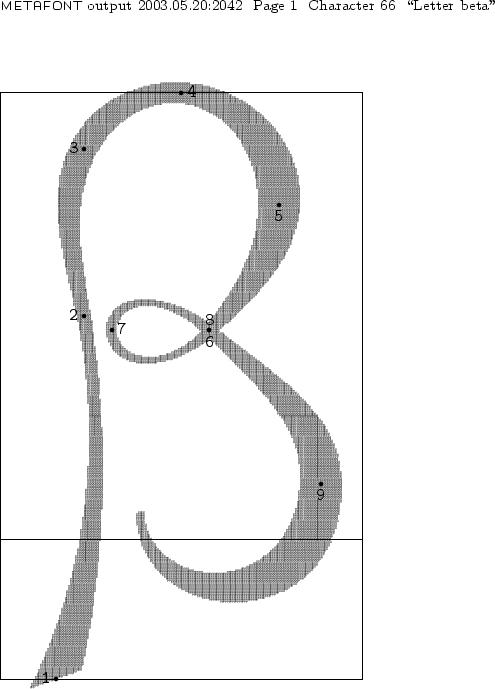
\includegraphics{beta.jpg}\\
The Greek letter \otherbeta.
\end{center}

To understand how \MF\ drew this figure out of the program you fed it with, let's have a closer
look at the program itself:\footnote{This is the reason why the program lines were numbered here.
\MF\ sources must \emph{never} have numbered lines and in future examples I won't include them.}

\begin{itemize}
\item Line~1 defines an algebraic parameter with which all the dimensions of the glyph will be
defined. By doing so, you will make it much easier to produce variants of your fonts, by changing
the values of a few parameters, rather than having to look through a full complicated source
where all the dimensions have been directly specified (one says ``hard-wired''), and as such
multiplying the chances you will make a mistake or will forget to change one value. Working with
parameters is the key ingredient to meta-design. This tutorial will slowly teach you to think
with parameters rather than direct values.
\item As you can see, in the first line the parameter ends in \verb|#|. However, in the rest
of the program, the parameter is simply called \verb|u|. What is happening here is that
``true'' lengths (i.e. device-independent values) in \MF\ are always specified with parameters
ending in \verb|#| (called ``sharped'' variables). However, to get the same values on all
devices (i.e. screens, different kinds of printers etc.), you need to specify which device
you create your font with, and then convert your ``sharped'' values into ``soft'',
device-dependent, values. That's what the \texttt{define\_pixels} command on Line~2 does. It
converts a ``sharped'' parameter into a ``soft'' one, of identical name but without a
\verb|#| sign at the end. This feature of \MF, related to the \emph{modes} you will learn
about in Lesson~3, is very much a sign of \MF's age, created at a time when printing devices were
far less flexible than they are now. Still, it is necessary to learn how it works, and it is
still useful for meta-design.
\item Line~3 indicates that we start now creating a character in the font. It defines the
position of the character in that font, as well as its dimensions (or rather the dimensions of an
abstract ``box'' around the character called the \emph{bounding box}, which is what
\TeX\ actually manipulates when it puts characters together on a page. This line also defines a
\emph{label} for this character (put just after the \texttt{beginchar} command between double
quotes), which appears on the proofsheets for this character. It is a good idea to always label
your characters, as it facilitates navigation in your programs.
\item Lines~4 to 11 define the positions of various points through which the ``pen'' will go to
draw the glyph. For now, just observe how all point positions are defined only in terms of the
parameter \verb|u| or of other points, rather than in terms of actual length values. This
makes the character easily scalable by just modifying the value of \verb|u#| once.
\item Lines~12 to 21 define \emph{pen positions}, i.e. the width of the pen at the position of
the point, and its inclination. This is what defines the looks of the character, compared to
similar characters using the same point positions.
\item Line~22 instructs \MF\ to take a certain pen (here with a thin round nib). It's with this
pen that \MF\ will draw the glyph. By changing the pen, you can achieve different kinds of
effects.
\item Line~23 is the actual (and only) drawing instruction. Its relative simplicity shows the
strength of \MF, which is able to interpolate the positions the pen has to go through between two
points without needing help from the user. Simply speaking, the command instructs \MF\ to draw
through all the different points in order, following the positions given by the different
\texttt{penpos} instructions, and creating the shape you can admire on the figure.
\item Line~24 instructs \MF\ to show, with their numbers, the points used for the construction of
the shape on the proofsheet. It is \emph{very} good practice to do so as much as possible.
\item Line~25 tells \MF\ that it has finished drawing the character, and that it can get ready to
draw another one, or to stop.
\item Line~26 instructs \MF\ that the job is finished and it can go home. Don't forget it, as
without it \MF\ will think there is still work to do and will wait patiently for you to feed it
with new instructions (\MF\ is a very obedient servant).
\end{itemize}

\noindent Once again, don't worry if you don't understand everything which is explained here.
The goal of this tutorial is after all to teach you what it means.

Now, you probably fell in love with the shape you just produced, and want to make a true font out
of it, in order to sprinkle your documents with \otherbeta eautiful \otherbeta etas.
To do so, go back to your command line, and enter the following line:

\begin{quote}
\begin{verbatim}
mf \mode=ljfour; mode_setup; input beta.mf
\end{verbatim}
\end{quote}

\noindent Some command lines give a special signification to the backslash character, and for
them the above line will probably result in an error.
If you get this error, just put quotes around the arguments of the \verb|mf| command, like this:

\begin{quote}
\begin{verbatim}
mf '\mode=ljfour; mode_setup; input beta.mf'
\end{verbatim}
\end{quote}

\noindent In the rest of this tutorial, I won't use quotes around such arguments, but feel free
to add them at need.
For now, just remember that the backslash indicates to \MF\ that it must expect
instructions on the command line rather than a filename, that the first two instructions put
\MF\ in true fontmaking mode\footnote{Depending on your installation, you may need to choose a
mode different from \texttt{ljfour}. Basically, you should choose the same that you used to
compile the gray font.} (rather than proofmode),
and that the last one causes \MF\ to finally load and compile \texttt{beta.mf}. The output you
will get should look like this:

\begin{quote}
\begin{verbatim}
This is METAFONT, Version 2.718281 (TeX Live 2013)
**\mode=ljfour; mode_setup; input beta.mf
(beta.mf [66] )
Font metrics written on beta.tfm.
Output written on beta.600gf (1 character, 436 bytes).
\end{verbatim}
\end{quote}

\noindent It is slightly different from the output you got the first time around, and indicates
that \emph{two} files have been created this time.
And indeed, if you check your directory, you should
see that a \texttt{beta.tfm} file and a \texttt{beta.600gf} (or similar with another number)
file have appeared. Now you still need to pack the \texttt{gf} file into a usable format. You do
so with this command:

\begin{quote}
\begin{verbatim}
gftopk beta.600gf beta.600pk
\end{verbatim}
\end{quote}

\noindent or this one:

\begin{quote}
\begin{verbatim}
gftopk beta.600gf beta.pk
\end{verbatim}
\end{quote}

\noindent if your platform needs unnumbered \texttt{pk} files. A \texttt{beta.600pk} or \texttt{beta.pk}
file should appear in your directory. And that's it! Your font is now available to every
\LaTeX\ document whose source is in the same directory as the font files
and you can test it with the following \LaTeX\ program:
\verbatiminput{letterbeta.tex}
Just compile it and check the result with your DVI viewer.
\end{exercise}

\chapter{My First Character}

Yes, we have already made our first character when we created \otherbeta.
For that character you just copied.
This time I am going to explain what goes into making a character.

\section{The command line}

Through most of this lesson we make use of the \MF\ command line and assume you are that will
display graphical results on your screen.
You are free to use text file and look at the \texttt{log} file, and create a proof sheet like
you did for \otherbeta eta.
If you are in a state where you are typing things in directly but don't have the ability to
results on screen, it can be helpful to know that if no name is provided the results are stored
in a set of files with the base name \texttt{mfput.}.
So we have \texttt{mfput.log}, $\ldots$

Open a command line, go to a useful directory, and start \MF\ by typing \verb|mf|.
You will receive a message like:

\begin{quote}
\begin{verbatim}
This is METAFONT, Version 2.718281 (TeX Live 2013)
**
\end{verbatim}
\end{quote}

\noindent The ``\verb|**|'' prompt indicates that \MF\ is expecting a filename.
We don't have a filename and just want to have a talk so we tell it to \verb|\relax| and receive
a new prompt of \verb|*| which means that \MF\ is ready to listen.
Go ahead and type the following (admittedly useless) line:

\begin{quote}
\begin{verbatim}
1+1;
\end{verbatim}
\end{quote}

\noindent \MF\ responds with:

\begin{quote}
\begin{verbatim}
>> 2
! Isolated expression.
<to be read again>
                   ;
<*> 1+1;

?
\end{verbatim}
\end{quote}

\noindent At the point the \verb|?| prompt is \MF\ asking what you want to do about it.
We are going to type \verb|s| which means to enter scrollmode --- when \MF\ sees an error it
reports it and just keeps on going.
Did you notice though, \MF\ correctly calculated the answer.
You can use this trick to have a handy (if talkative) desk calculator --- Knuth claims to
sometimes do this.

Now try entering the following:

\begin{quote}
\begin{verbatim}
*1+1; 2-1; 2*3; 3/2; 3div2; 3mod2; 2**3;
\end{verbatim}
\end{quote}

\noindent The beginning of the output looks like this:

\begin{quote}
\begin{verbatim}
>> 2
! Isolated expression.
<to be read again>
                   ;
<*> 1+1;
         2-1; 2*3; 3/2; 3div2; 3mod2; 2**3;
>> 1
\end{verbatim}
\end{quote}

\noindent First we get the answer to $1+1$, later we receive a line where the second line begins with
\texttt{2-1;} and the answer to $2-1$ is just below it.
These are our most common operators.

\begin{enumerate}
\item[\texttt{+}]   means to add two values;
\item[\texttt{-}]   means to subtract two values;
\item[\texttt{*}]   means to multiply two values;
\item[\texttt{/}]   means to divide two values;
\item[\texttt{div}] means to divide two values and throw away any fractional part;
\item[\texttt{mod}] means to divide two values and report on the remainder; and
\item[\texttt{**}]  means to exponate two numbers (so 2**3 is $2^3$).
\end{enumerate}

\noindent You can get roots by using \verb|**| and a fraction.
So \verb|2**(1/4);| will give you the fourth root of 2.

There are limits, only about four digits to the right of the decimal point are accurate, and
\MF\ has a maximum value of about thirty-two thousand.
Try this out and see what \MF\ answers you.

\begin{quote}
\begin{verbatim}
2**10; 2**11; 2**16; 2**17;
\end{verbatim}
\end{quote}

The correct answers are $1 024$, $2 048$, $32 768$, and $65 536$.
The first three are correct, if we round the fifth digit properly, and the last one is just plain
wrong.
The value $32 787.999 98$ means ``$\infty$'' and \MF\ refuses to go past $\infty$.

Finally, did you notice I said two \emph{values} and not two \emph{numbers}.
\MF\ can work with more that just simple numbers, and many of these operators are valid for
points, vectors, and angles.

\section{Some simple algebra}

\MF\ can also do quite a bit of algebra --- by which we mean keep track of relationships and
manipulate them to solve for unknown values.
For most programming languages when you see \verb|c=a| it means that \verb|c| is going to be
assigned the value that \verb|a| has \emph{at that moment in time}.
This is why some languages, like Pascal and Ada use \verb|:=| instead.
When you type \verb|c:=a| it is supposed to visually remind you of $c\leftarrow a$.
When you type \verb|c=a| in Ada it means you are comparing two values for equality.

\MF\ also maintains this distinction, but it can much more than just compare values.
First, let's make a pair of assignments.

\begin{quote}
\begin{verbatim}
tracingequations:=tracingonline:=1;
\end{verbatim}
\end{quote}

These variables start out with values of $0$ and by changing them to $1$ we are asking \MF\ to
tell us about its thought processes as it works.
Now let's continue.

\begin{quote}
\begin{verbatim}
a+b-c=0;
\end{verbatim}
\end{quote}

\noindent And \MF\ tells us:

\begin{quote}
\begin{verbatim}
## c=b+a

*
\end{verbatim}
\end{quote}

\noindent So we told \MF\ that \verb|a+b-c| has a relationship of equality to zero.
Whatever those three values are, that result must add up to zero.
Then \MF\ told us that it doesn't know what \verb|a| or \verb|b| are but it did determine that
\verb|c=b+a|.
It could just as well determined that \verb|b=c-a| or anything else.
This is just how \MF\ wants to remember this relationship.
Now let's give it a little more information.

\begin{quote}
\begin{verbatim}
c=2a;
\end{verbatim}
\end{quote}

\noindent\MF\ now knows that if \verb|c=b+a| \emph{and} \verb|c=2a| then \verb|b| must have the same value
as \verb|a|, which is why it tells us \verb|## b=a|.
If you are used to programming traditional imperative languages, it may strike you as a bit off.
But we didn't say \verb|:=| to make an assignment, we provided an additional relationship.
Also notice that you did not have to say \verb|c=2*a;|, because \MF\ can distinguish between
numbers and variables and known that $2x$ means $2\cdot x$ or $2\times x$.

Let's give \MF\ just a little more information.
Tell \MF\ that \verb|a=5;| and see what it says.
First it reports that it took in your relationship and internally stored it \verb|## a=5|.
Remember that it already figured out that \verb|b=a| so the next thing it reports to us is that
\verb|#### b=5|.
Finally, it also knows that \verb|c=b+a| \emph{and} \verb|c=2a| so \verb|#### c=10|.

Let's give \MF\ just a little bit more information.
Tell \MF\ that \verb|c=0;| and it reports:

\begin{quote}
\begin{verbatim}
! Inconsistent equation (off by -10).
<to be read again>
                   ;
<*> c=0;
\end{verbatim}
\end{quote}

It already knows that \verb|c=10| so it can't also be true that \verb|c=0| and it rightfully
complained.
You can tell it \verb|c:=0;| and it will happily forget everything it already knows about
\verb|c| and report that it has a value of $0$.
So be careful about whether you are assigning or establishing an algebraic relationship.

\begin{exercise}
Here is a system of equations, presented in a mathematical way:
\begin{displaymath}
\left\{ \begin{array}{r@{}c@{}r@{}c@{}r@{}c@{}r}
a&+&b&+&2c&=&3\\
a&-&b&-&2c&=&1\\
 & &b&+& c&=&4
\end{array}\right.
\end{displaymath}
\begin{itemize}
\item Use \MF\ to find out if this system of equations is consistent.
\item Is there enough information to solve them?
\item If so, what are the values?
\end{itemize}

\answerhead
\answerline{If you type the equations in correctly, \noexpand\MF\ does not complain so the
equations are consistent}
\answerline{You can either use the trick we used, or you can type in the equations and follow up
with {\noexpand\tt a; b; c;}.}
\answerline{\noexpand\MF\ will report values of $2$, $7$, and $-3$ so there is enough information
to solve them.}
\end{exercise}

\section{Co\"ordinates, lines, and curves}

Having a desk calculator is convenient.
Having a limited computer algebra system is nice.
But how do we draw?

Our first non-number value\footnote{Remember me saying that the operators worked for more than
numbers?} is the co\"ordinate.
A co\"ordinate is a pair of values representing horizontal and then vertical direction.
So if we say \verb|(3,2)| we mean start at some predefined location, move three units
horizontally (to the right) and two units vertically (up).
The predefined location is called the \textbf{origin} because it is where all direction is
measured from.

If the first number is:
\begin{center}
\begin{tabular}{cl}
$>0$&the horizontal movement is right;\\
$=0$&there is no horizontal movement; and\\
$<0$&the horizontal movement is left.\\
\end{tabular}
\end{center}

In a similar way if the second number is:
\begin{center}
\begin{tabular}{cl}
$>0$&the vertical movement is up;\\
$=0$&there is no vertical movement; and\\
$<0$&the vertical movement is down.\\
\end{tabular}
\end{center}

So where are these co\"ordinates measuring distance?
\MF\ has some graph paper that it keeps track of internally.
This is a grid of square \textbf{pixels}, or \emph{picture elements}.
So let's try a bit of these.

\begin{quote}
\begin{verbatim}
showit;
drawdot(35,70); showit;
drawdot(65,70); showit;
draw(20,100)--(50,125)--(80,100); showit;
draw(20,40)..(50,25)..(80,40); showit;
shipit;
end
\end{verbatim}
\end{quote}

I chose that breakdown of commands so that you could watch the drawing happen.
The first \verb|showit;| is just to bring up a visual display if your system's \MF\ happens to
support one.
Some systems will not require this, others seem to need this to show the first \verb|drawdot|
command.
Just like with \verb|\relax|, I will not include it in other instructions, so if you forget you
may need to do \verb|showit;|
twice after your first draw instruction.
After each \verb|drawdot| command you saw a dot appear.
The second dot was to the right of the first dot because the first number (the horizontal
position) was more positive.
The \verb|draw| command with \verb|--| drew a line.
The \verb|draw| command with \verb|..| drew a curved line.
When you entered \verb|shipit;|, \MF\ responded with \verb|[0]| which means that it assigned the
current state of the graph paper to character $0$.
Finally, \verb|end| told \MF\ you were done and it reported that it created a font called
\texttt{mfput.2062gf}.
If you use \texttt{gftodvi} and take a look, you will find that there is one page and the
character is

\begin{center}
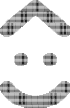
\includegraphics{smiley.png}
\end{center}

\noindent So we have two points, a bent line, and a nice curve.
But what are lines and curves really?
A line is a set of two or more points that \MF\ has been told to connect as if using a straight
edge.
A curve is a set of two or more points that \MF\ has been told to freehand draw through.
``Freehand draw'' sounds a bit fuzzy, and \MF\ is actually very exacting about the type of curve
it draws; but the intent is for \MF\ to draw as if it was doing a freehand curve.

So lines and curves are sets of two or more connected co\"ordinates.
Let's try this out.

\begin{quote}
\begin{verbatim}
*draw(0,0)--(0,100); showit;
*draw(100,0)..(100,100); showit;
\end{verbatim}
\end{quote}

\MF\ is very exacting about what a curve should look like, and if a curve only has two
co\"ordinates then it is actually a line.

\section{Co\"ordinates as variables}

So far I keep promising that \MF\ can work with more than numbers, but I keep not doing it.
So let's start with how do we assign co\"ordinates to a variable.

By long established tradition that predates \MF, the first number of a co\"ordinate is called $x$.
By the same tradition, the second number of a co\"ordinate is called $y$.
In keeping with that tradition \texttt{x<number>} represents the first number of a co\"ordinate,
and \texttt{y<number>} represents the second number of a co\"ordinate.
So if we wanted to define a rectangle we could say \verb|x1=0; y1=0; x2=50; y2=0;| $\ldots$
Which probably feels like a cheat after all of my promises.
Since \MF\ treats $x$ as the horizontal movement and $y$ as vertical movement, it was decided
that $z$ would be a coordinate.
And now we can finally use a coordinate as a variable.
\verb|z1=(0,0);| \verb|z2=(100,0);| \verb|z3=(100,50);| \verb|z4=(0,50);|
\verb|draw z1--z2--z3--z4--z1;| \verb|showit;| and you will have a nice rectangle.

\section{Co\"ordinate algebra}

This is how we begin to introduce some meta-ness to \MF.
It's perfectly fine to say ``I want a rectangle and I want it to have these corners.''
But you can also tell \MF\ things like ``I want a rectangle that is twice as wide as it is high.''

\begin{quote}
\begin{verbatim}
x1=x2; x3=x4;
y2=y3; y4=y1;
y2-y1=2*(x3-x1);
z1=(0,0);
x3=100;
draw z1--z2--z3--z4--z1;
showit;
\end{verbatim}
\end{quote}

I do want to point out that there is no requirement to draw the points in order.
\MF\ will not complain if you say \verb|draw z2--z4--z1--z3--z1;|.
The reason for them to go in order is for \emph{our} convenience.

Now if we understand the writing system we are trying to create well enough, we can add relationships
between co\"ordinates and ensure things like a capital H has stems with equal widths.
We can even assign a value to a \textbf{parameter} like \verb|stem_width| and use that is making
all of our letters to ensure that all stems have equal width.

If you know anything about font design, you will have realized that I just lied.
There are going to be cases where some stems will need to be slightly narrower or slightly
wider than the \emph{design}'s stem width.
It still holds true that we can make all the stem widths \emph{appear} equal because just like I
stated \verb|y2-y1=2*(x3-x1);| I could have just as easily said
\verb|y2-y1=0.95*stem_width;| and had uneven stem widths that look even.\footnote{If you aren't
familiar with font design this may seem strange, but well designed fonts are created to account
for the various optical illusions we all see and make the letter look correct anyway.}

\section{Line algebra}

This all works well for parallel figures like squares and rectangles, what about more complicated
shapes like the ones we find in letters?
We can use the $z$ co\"ordinate to find things part way across a line.
Consider the capital letter A.
We know we want the horizontal line to connect from one line to the other.
How do we find the exact co\"ordinate to do that?
We don't.

Lets imagine that we have defined \verb|z1|, \verb|z2|, and \verb|z3| to be the bottom-left, the
top, and the bottom right of a capital A.
We want to define \verb|z4| and \verb|z5| to control the horizontal bar and we want to have it be
exactly about 70\% of the way up.

\begin{quote}
\begin{verbatim}
z4 = z1+0.7(z2-z1);
z5 = z2+0.7(z3-z2);
\end{verbatim}
\end{quote}

\noindent Treating points across a line like this has a well established practice in mathematics
and is called \emph{parameterization} of a line.
\MF\ uses this and you can instead say:

\begin{quote}
\begin{verbatim}
z4=0.7[z1,z2];
z5=0.7[z2,z3];
\end{verbatim}
\end{quote}

In this case \verb|0.7[z1,z2]| means ``as you move from \verb|z1| to \verb|z2|, find the point
$0.7$ times the length.''
And you are not required to only use numbers less than one.
You can also use this to define points twice as far or even the opposite direction.

\section{Let's draw some characters}

This section is all assignments.
You should have seen enough to look over the last several sections and figure out how to define
these shapes.

For each of these exercises, create a separate \texttt{mf} file so that you can get a clean
painting service each time.
Just name them \texttt{e3.mf}, \texttt{e4.mf}, and so on.
Just like the first exercises, I don't have an answer here.
The answer is the process of doing this.

\begin{exercise}
Pick some co\"ordinates and have \MF\ draw a capital letter E.
\end{exercise}

\begin{exercise}
This time, establish the correct relationships between $x$s and $y$s.
For instance, the two $y$ co\"ordinates of the top line for the letter E are equal.
\end{exercise}

\begin{exercise}
Now make the middle horizontal line of the E be 90\% of the length of the top and bottom lines.
(The $x$ co\"ordinates of your top and bottom lines are related because of the last exercise, right?)
\end{exercise}

\begin{exercise}
Now make the middle horizontal line of the E to be exactly in the middle.
(Unless you already did that.)
\end{exercise}

That's it for this lesson.
In the next lesson we'll learn how to make our lines a little more interesting.

\chapter{Pens and Curves}

\section{Back to arithmetic}

In lesson one I mentioned that we had operators which operated on values, but I did not say which
operators worked on which types.
Now we will talk about the operators, what they work on, and even cover a new data type.

Before we get into any of that we should discuss a few other \emph{numbers} that \MF\ knows about.
These are \verb|down|, \verb|epsilon|, \verb|infinity|, \verb|left|, \verb|origin|, \verb|right|,
\verb|up|, and \verb|whatever|.

\begin{itemize}
\item[\texttt{down}] is a co\"ordinate.
It's value is $(0,-1)$.
It is used to point portions of a curve down.
\item[\texttt{epsilon}] is a number.
It's value is $\frac{1}{65536}$ which is the smallest non-zero number that \MF\ can work with.
It is used when you want something to change just the tiniest bit.
\item[\texttt{infinity}] is a number.
It's value is $32 767 \frac{65535}{65536}$ and is the largest number that \MF\ can work with.
Operators will tap out at $\infty$ and $-\infty$ to avoid overflow.
\item[\texttt{left}] is a co\"ordinate.
It's value is $(-1,0)$.
It is used to point portions of a curve left.
\item[\texttt{origin}] is a co\"ordinate.
It's value is $(0,0)$.
It is used to get portions of a curve to behave as a start or end point.
\item[\texttt{right}] is a co\"ordinate.
It's value is $(1,0)$.
It is used to point portions of a curve right.
\item[\texttt{up}] is a co\"ordinate.
It's value is $(0,1)$.
It is used to point portions of a curve up.
\item[\texttt{whatever}] is a number.
It deliberately has no value.
It is used when a value is needed but you don't care what the value is.
\end{itemize}

There is one new data type to consider --- well half of a data type.
The \emph{angle} is a number which can be interpreted as a quantity of degrees.
$0$ degrees is to the right, $90$ degrees is up, and so forth.
This allows us to set the angle of lines and also to test for things like are lines parallel or
perpendicular.

Before I get to the operators, I want to pre-emptively answer a question I'm sure to hear.
``Why are you not covering all the cool things you can do with all of these functions?''
One, I did say to get and read \textsl{The \MF book} which describes each of these in detail.
Two, my audience is people trying to play around enough to make conscripts for their conlangs.
Knowing all the things you can do with \verb|rotatedabout| is really helpful when making fonts
for well established writing systems.
But that's not my audience.
Instead, I will just cover each of these briefly and leave a deeper level of playing to my
readers.

``Doesn't that mean that they are more likely to just draw lines and not be meta?''
So what?
After the writing has become established, go back and be meta.
When first inventing orthographies you don't need to be meta.
You need the freedom to play.
And that's what I am offering.
In fact our next lesson will start \emph{re}inventing writing systems.

Now let's list all the operators, what they work on, and what they do.
When we say ``number'' we mean ``number or angle''.
When we say ``pair'' we mean ``co\"ordinates or pair''.

\noindent
\hangindent 7 mm
\textbf{\tt +} works with either two numbers or two pairs.\\
Examples:
\begin{tabular}{ll}
\verb|1+2;|&\verb|(1,2)+(3,4)|\\
\verb|3|&\verb|(4,6)|\\
\end{tabular}\\
Function: Add.

\noindent
\hangindent 7 mm
\textbf{\tt -} works with either two numbers or two pairs.\\
Examples:
\begin{tabular}{ll}
\verb|1-2;|&\verb|(1,2)-(3,4);|\\
\verb|-1|&\verb|(-2,-2)|\\
\end{tabular}\\
Function: Subtract.

\noindent
\hangindent 7 mm
\textbf{\tt *} works with either two numbers or a pair and number.\\
Examples:
\begin{tabular}{ll}
\verb|1*2|&\verb|(1,2)*3|\\
\verb|2|&\verb|(3,6)|\\
\end{tabular}\\
Function: Multiply.

\noindent
\hangindent 7 mm
\textbf{\tt /} works with two numbers or a pair and a number.\\
Examples:
\begin{tabular}{ll}
\verb|1/2|&\verb|(1,2)/3|\\
\verb|0.5|&\verb|(0.33333,0.66667)|\\
\end{tabular}\\
Function: Divide.

\noindent
\hangindent 7 mm
\textbf{\tt **} works with two numbers.\\
Examples:
\begin{tabular}{l}
\verb|1**2;|\\
\verb|1|
\end{tabular}\\
Function: Exponeation or power.

\noindent
\hangindent 7 mm
\textbf{\tt =} works with matching types.\\
Examples:
\begin{tabular}{ll}
\verb|x1=3;|&\verb|z1=(1,2);|\\
\end{tabular}\\
Function: Equality.

\noindent
\hangindent 7 mm
\textbf{\tt abs} works with a number or pair.\\
Examples:
\begin{tabular}{ll}
\verb|abs 1;|&\verb|abs (1,2);|\\
\verb|1|&\verb|2.23607|\\
\end{tabular}\\
Function: Absolute value or length.

\noindent
\hangindent 7 mm
\textbf{\tt angle} works with a pair.\\
Examples:
\begin{tabular}{l}
\verb|angle (1,2);|\\
\verb|63.43495|\\
\end{tabular}\\
Function: Find the angle.

\noindent
\hangindent 7 mm
\textbf{\tt ceiling} works with a number.\\
Examples:
\begin{tabular}{l}
\verb|ceiling 1.2|\\
\verb|2|\\
\end{tabular}\\
Function: round up.

\noindent
\hangindent 7 mm
\textbf{\tt cosd} works with a number.\\
Examples:
\begin{tabular}{l}
\verb|cosd 1;|\\
\verb|0.99985|\\
\end{tabular}\\
Function: cosine from degrees.

\noindent
\hangindent 7 mm
\textbf{\tt dir} works with a number.\\
Examples:
\begin{tabular}{l}
\verb|dir 1;|\\
\verb|(0.99985,0.01746)|\\
\end{tabular}\\
Function: Unit direction.

\noindent
\hangindent 7 mm
\textbf{\tt div} works with two numbers.\\
Examples:
\begin{tabular}{l}
\verb|3 div 2;|\\
\verb|1|\\
\end{tabular}\\
Function: Integer divide.

\noindent
\hangindent 7 mm
\textbf{\tt dotprod} works with two numbers or two pairs.\\
Examples:
\begin{tabular}{ll}
\verb|1 dotprod 2;|&\verb|(1,2) dotprod (3,4);|\\
\verb|4|&\verb|11|\\
\end{tabular}\\
Function: Dot product.

\noindent
\hangindent 7 mm
\textbf{\tt floor} works with number.\\
Examples:
\begin{tabular}{l}
\verb|floor 1.2;|\\
\verb|1|\\
\end{tabular}\\
Function: round down.

\noindent
\hangindent 7 mm
\textbf{\tt length} works with number or pair.\\
Examples:
\begin{tabular}{ll}
\verb|length -1|&\verb|length (1,2);|\\
\verb|1|&\verb|2.23607|\\
\end{tabular}\\
Function: Absolute value or length.

\noindent
\hangindent 7 mm
\textbf{\tt max} works with set of numbers.\\
Examples:
\begin{tabular}{ll}
\verb|max (1,2);|\verb|max (1,2,3);|\\
\verb|2|&\verb|3|\\
\end{tabular}\\
Function: Maximum.

\noindent
\hangindent 7 mm
\textbf{\tt min} works with set of numbers.\\
Examples:
\begin{tabular}{ll}
\verb|min (1,2);|\verb|min (1,2,3);|\\
\verb|1|&\verb|1|\\
\end{tabular}\\
Function: Minimum.

\noindent
\hangindent 7 mm
\textbf{\tt mod} works with two numbers.\\
Examples:
\begin{tabular}{l}
\verb|3 mod 2;|\\
\verb|1|\\
\end{tabular}\\
Function: Modulus or remainder

\noindent
\hangindent 7 mm
\textbf{\tt reflectedabout} works with three pairs.\\
Examples:
\begin{tabular}{l}
\verb|(x, y) reflectedabout (z1, (0, 0))|\\
\end{tabular}\\
Function: Reflect image element.

\noindent
\hangindent 7 mm
\textbf{\tt rotated} works with number.\\
Examples:
\begin{tabular}{l}
\verb|rotated 90;|\\
\end{tabular}\\
Function: Rotate image element.

\noindent
\hangindent 7 mm
\textbf{\tt rotatedaround} works with pair and number.\\
Examples:
\begin{tabular}{l}
\verb|rotatedaround (z1, 90);|\\
\end{tabular}\\
Function: Rotate image element around a point.

\noindent
\hangindent 7 mm
\textbf{\tt round} works with number or pair.\\
Examples:
\begin{tabular}{ll}
\verb|round 1.2;|&\verb|round (1.2,3.4);|\\
\verb|1|&\verb|(1,3)|\\
\end{tabular}\\
Function: Round to nearest.

\noindent
\hangindent 7 mm
\textbf{\tt scaled} works with a pair and a number.\\
Examples:
\begin{tabular}{l}
\verb|(1,2) scaled 3;|\\
\verb|(3,6)|\\
\end{tabular}\\
Function: Scale or multiply.

\noindent
\hangindent 7 mm
\textbf{\tt shifted} works with two pairs.\\
Examples:
\begin{tabular}{l}
\verb|(1,2)+(3,4)|\\
\verb|(4,6)|\\
\end{tabular}\\
Function: Shift or add.

\noindent
\hangindent 7 mm
\textbf{\tt sind} works with number.\\
Examples:
\begin{tabular}{l}
\verb|sind 1;|\\
\verb|0.01746|\\
\end{tabular}\\
Function: sine from degrees.

\noindent
\hangindent 7 mm
\textbf{\tt sqrt} works with number.\\
Examples:
\begin{tabular}{l}
\verb|sqrt 1|\\
\verb|1|\\
\end{tabular}\\
Function: square root.

\noindent
\hangindent 7 mm
\textbf{\tt xscaled} works with a pair.\\
Examples:
\begin{tabular}{l}
\verb|(1,2) xscaled 3;|\\
\verb|(3,2)|\\
\end{tabular}\\
Function: multiply first number of pair.

\noindent
\hangindent 7 mm
\textbf{\tt yscaled} works with a pair.\\
Examples:
\begin{tabular}{l}
\verb|(1,2) yscaled 3;|\\
\verb|(1,6)|\\
\end{tabular}\\
Function: multiply second number of pair.

\section{Curved lines}

Curved lines, also simply called \emph{curves}, are lines which are not straight.
We saw examples of both straight and curved lines during an earlier lesson.
In this tutorial, as you have probably guessed by now, I usually reserve the word ``line'' to
refer to straight lines only, and use the word ``curve'' for curved ones.
This is why you would generally find me saying things like ``line or curve''.
This is different from the usual use of the word ``line'', which in common speech refers to any
kind of line.

Let's review the two commands we used to get our smiley eyebrows and mouth in the earlier lesson.

\begin{quote}
\begin{verbatim}
draw(20,100)--(50,125)--(80,100);
draw(20,40)..(50,25)..(80,40);
\end{verbatim}
\end{quote}

Notice that the \texttt{draw} command takes a series of co\"ordinates and then draws either a
line or a curve between sets of co\"ordinates.
You can even mix and match between them which is helpful for letters like the capital B which are
a mix of straight and curved lines.
Let's try that out.
Start up \MF and try the following to see what the result is.

\begin{quote}
\begin{verbatim}
draw(20,40)--(50,25)..(80,40); showit;
\end{verbatim}
\end{quote}

Two straight lines!
You can mix and match, but if you only have two points connecting a curve, you get a line instead.
Try this version instead.

\begin{quote}
\begin{verbatim}
draw(20,40)--(50,25)..(80,40)..(110,25);
\end{verbatim}
\end{quote}

For the rest of this lesson, I'm going to assume that you have a good grasp of lines and focus
more on making curves.

\begin{framed}
Once again I am extremely indebted to \textsl{The \MF tutorial} by Christophe~Grandsire for the
remainder of this lesson.
I tried doing the remainder of this lesson in a few different ways and just found he did the job
so well that I could not improve upon it.
\end{framed}

\noindent
This is the very secret of the powerful \texttt{draw}
command of \MF. You can feed it with any number of coordinate pairs (always separated two by two
with ``..''), and it will draw a smooth curve passing by \emph{all} those points (in the order
you typed them in) as well as it can!

\begin{center}
\begin{tabular}{cc}
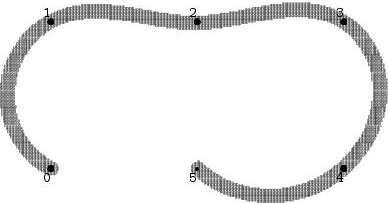
\includegraphics[width=0.3\textwidth]{curve1.jpg} & 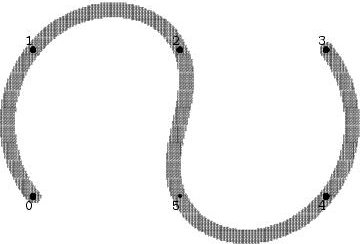
\includegraphics[width=0.3\textwidth]{curve2.jpg} \\
\texttt{draw z0..z1..z2..z3..z4..z5;} & \texttt{draw z0..z1..z2..z5..z4..z3;} \\
(a) & (b) \\
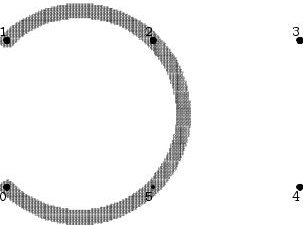
\includegraphics[width=0.3\textwidth]{curve3.jpg} & 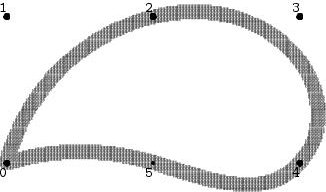
\includegraphics[width=0.3\textwidth]{curve4.jpg} \\
\texttt{draw z0..z5..z2..z1;} & \texttt{draw z0..z5..z4..z2..z0;} \\
(c) & (d) \\
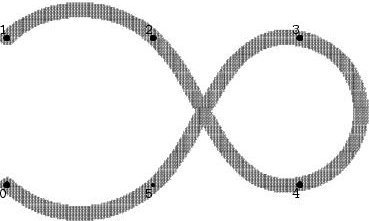
\includegraphics[width=0.3\textwidth]{curve5.jpg} & 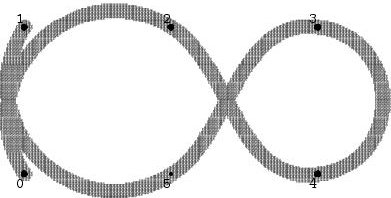
\includegraphics[width=0.3\textwidth]{curve6.jpg} \\
\texttt{draw z0..z5..z3..z4..z2..z1;} & \texttt{draw z0..z2..z4..z3..z5..z1;} \\
(e) & (f) \\
\end{tabular}\\
Examples of curves and the commands that drew them.
\end{center}

As you see in those examples, \MF\ doesn't mind bending the curve quite a lot to get a very
smooth result. That's because as it is used right now, it will always construct curves where
bending is \emph{minimal} at the positions of the given points.
Another rule that \MF\ uses when it draws curves is that between two
consecutive points given in the \texttt{draw} command, it will try to draw a curve
\emph{without} inflection point, i.e. a curve which bends in one direction only.\footnote{an
inflection point is a position on a curve where bending changes direction. It's where a curve
changes from concave to convex or the other way around. The middle of the
letter S is a good example of inflection point.} \MF\ will break this rule only when it has no
other way to keep the curve smooth (as in (b)). This explains why in (f), \MF\ drew such a large
loop between points 0 and 2, and between points 5 and 1. A more direct curve between those points
would have created an inflection point, and there was a better (in \MF's point of view) way to
keep a smooth curve. On the other hand, \MF\ has no problem creating an inflection point at the
position of a point given in the \texttt{draw} command. Look for instance at point 5 of (d). Try
to remember those two drawing rules. They will help you correctly translate the curves you want
to draw into \MF\ instructions.

The \texttt{draw} instruction is very powerful. However, if you have tried your hand at a few
curves, you have probably noticed that it is sometimes \emph{too} powerful, in the sense that
\MF\ makes decisions about the shape of the curve you want to draw which are against what you
meant. That's actually logical: giving just the position of a few points is quite little
information, and \MF\ cannot read your mind! From the positions of the points you gave,
it will try to make a nice and smooth curve, but that will be according to its own criteria,
since it has no way to guess yours. The result is that it will sometimes draw things differently
from what you expected.

So does that mean that \MF\ is the boss and that we can only accept its ideas and hope that they
sometimes look enough like ours? Of course not! \MF\ is just a computer program, and will do as
\emph{we} want, if we \emph{tell} it to obey us. In other words, if you want \MF\ to draw exactly
the curve you want it to draw, you'll have sometimes to give it more information than just the
positions of the points. How do we do that? Well, there are various ways, and we will see only
two of them in this lesson. We will learn more about those methods of control in later lessons.

The most obvious way to control the shape of a curve is to specify its direction (or \emph%
{slope}) at some point(s). \MF\ allows you to specify the direction the curve will take when it
passes by the points you use to define your curve (in other words, in order to control the slope
of the curve at some position, you need to put the coordinates of that position in your \texttt%
{draw} command). Specifying the direction itself is easy when you remember that coordinate pairs
aren't only used to define point positions, but can also be used to define vectors, i.e.
displacements. And since displacements are always done according to a definite direction, using
vectors to specify directions is just natural. And indeed, to specify a direction at some point
named \verb|z| in your \texttt{draw} command, you just need to put a coordinate pair, which
will be interpreted as a vector, in curly braces ``\{\}'', and put the whole thing next to
\verb|z| (nothing can go in between, especially not ``..''!). Here is how this syntax looks
like:

\begin{quote}
\texttt{draw} \emph{$<$something$>$}\texttt{..\{(}\emph{a}\texttt{,}
\emph{b}\texttt{)\}z..}\emph{$<$something else$>$}\texttt{;}
\end{quote}

\noindent or

\begin{quote}
\texttt{draw} \emph{$<$something$>$}\texttt{..z\{(}\emph{a}\texttt{,}
\emph{b}\texttt{)\}..}\emph{$<$something else$>$}\texttt{;}
\end{quote}

\noindent where (\emph{a}, \emph{b}) is a coordinate pair defining a vector. For now, don't
worry about the position of the \texttt{\{(}\emph{a}\texttt{,} \emph{b}\texttt{)\}} part.
It doesn't change anything
if you put it before or after the point coordinates (note, however, that if you put such a
direction specification with the \emph{first} point coordinates of your \texttt{draw}
instruction, you can only add it \emph{after} the point coordinates. A syntax like:

\begin{quote}
\texttt{draw \{(}\emph{a}\texttt{,} \emph{b}\texttt{)\}z..}\emph{$<$something$>$}\texttt{;}
\end{quote}

\noindent will result in an error).

Now, you may think that it's great, but defining directions with pair coordinates is not that
simple. After all, you probably can't see at first sight what direction corresponds to a vector
of coordinates ($-$5.8, 12.3), and what vector corresponds to a direction at 13.5$^\circ$ up
from the horizontal, pointing to the left. Well, it's time then to remember the
series of
predefined pair values and operators which are there to take care of this job. If you need a
simple direction, use the vectors \texttt{up}, \texttt{down}, \texttt{left} and \texttt%
{right}, whose names correspond exactly to the directions they define. Remember also that if you
have two points labeled 1 and 2, \texttt{z2 - z1} is the vector corresponding to the
displacement between point 1 and point 2, in the direction of point 2. You can use this at your
advantage if you want to force a curve to go in the direction defined by those two points. And
finally, if you know the angle the direction you want the curve to take has with the horizontal,
don't hesitate to use ``\texttt{dir}'' to create a unit vector defining that direction. As you
see, you already have all the tools necessary to define directions without having to know exactly
how to relate the coordinates of a vector to the direction it defines.

\begin{exercise}
Answer the following questions as precisely as possible:
\begin{enumerate}
\item What is the difference between the directions defined by \texttt{\{left\}} and \texttt%
{\{right\}}?
\item What direction is defined by \texttt{\{up} + \texttt{right\}}?
\item What is the difference between the directions defined by \texttt{\{up\}} and \texttt%
{10\{up\}}?
\end{enumerate}

\answerhead
\answerline{\noexpand\begin{enumerate}}
\answerline{\noexpand\item {\noexpand\tt\char"7B left\char"7D} and {\noexpand\tt \char"7B
right\char"7D} both define a horizontal direction, and thus will force the curve to be horizontal
at the point where they are specified.}
\answerline{But {\noexpand\tt\char"7B left\char"7D} also indicates that the curve will have to go
from right to left when it passes the specified point, while {\noexpand\tt\char"7B right\char"7D}
forces the curve to go from left to right at that point.}
\answerline{So {\noexpand\tt\char"7B left\char"7D} and {\noexpand\tt\char"7B right\char"7D}
define both horizontal directions, but of opposite {\noexpand\it sense}.}
\answerline{Check out the curves below to see what tremendous consequences the difference of
sense can have for the overall shape of a curve.}
\answerline{}
\answerline{\noexpand\begin{center}}
\answerline{\noexpand\begin{tabular}{cc}}
\answerline{\noexpand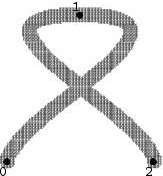
\includegraphics{leftdir.jpg} &}
\answerline{\noexpand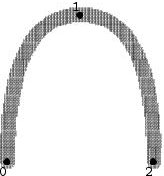
\includegraphics{rightdir.jpg} \noexpand\\}
\answerline{{\noexpand\tt draw z0\char"7B up\char"7D..\char"7B left\char"7D z1..\char"7B
down\char"7D z2;} &}
\answerline{{\noexpand\tt draw z0\char"7B up\char"7D..\char"7B right\char"7D z1..\char"7B
down\char"7D z2;} \noexpand\\}
\answerline{\noexpand\end{tabular}\noexpand\\}
\answerline{An example illustrating the difference between {\noexpand\tt\char"7B left\char"7D} and
{\noexpand\tt\char"7B right\char"7D}.}
\answerline{\noexpand\end{center}}
\answerline{}
\answerline{\noexpand\item {\noexpand\tt up} is a vector meaning: ``move 1 pixel upwards'', while
{\noexpand\tt right} means: ``move 1 pixel to the right''.}
\answerline{If you remember that the addition of vector is simply the addition of displacements
one after the other, {\noexpand\tt up} + {\noexpand\tt right} means: ``move 1 pixel upwards then
1 pixel to the right.''}
\answerline{You can check on some graph paper that this corresponds to the direction exactly in
between the upwards and rightwards directions, i.e. at 45$^\circ$ from the horizontal, pointing
to the right.}
\answerline{In other words, writing {\noexpand\tt\char"7B up + right\char"7D} is exactly
equivalent to writing {\noexpand\tt\char"7B dir 45\char"7D}.}
\answerline{\noexpand\item None!}
\answerline{The direction a vector defines is independent from its length ({\noexpand\tt up} and
{\noexpand\tt 10up} both point exactly upwards, regardless of the fact that one is 10 times as
long as the other), so {\noexpand\tt\char"7B up\char"7D} and {\noexpand\tt\char"7B 10up\char"7D}
both define exactly the same direction.}
\answerline{This means that you needn't worry about the length of your vectors when you define
directions will just be ignored by \noexpand\MF.}
\answerline{Just make sure your vector {\noexpand\it does} have some length.}
\answerline{A vector of length 0 like {\noexpand\tt origin} cannot define any direction, and thus
something equivalent to {\noexpand\tt \char"7B origin\char"7D} will just be ignored by
\noexpand\MF.}
\answerline{(at least the length of the resulting vector, when it results from a calculation.}
\answerline{But inside the calculation the lengths of the vectors are meaningful: {\noexpand\tt
up} + {\noexpand\tt right} defines a different direction from {\noexpand\tt 10up + right}).}
\answerline{\noexpand\end{enumerate}}
\end{exercise}

\begin{exercise}
We have four points, labeled from 0 to 3, whose respective coordinates are given by the
following lines:

\begin{quote}
\begin{verbatim}
z0 = (0, 0);
z1 = (100, 100);
z2 = (50, 60);
z3 = (120, 10);
\end{verbatim}
\end{quote}

\noindent We want to draw a curve going from point 0 to point 1, passing exactly by the middle
between points 2 and 3 and being at that point perpendicular to the line defined by those points
2 and 3. Write the instructions necessary to define the middle point between points 2 and 3 (that
you will label 4) and to draw the wanted curve (\emph{hint}: you only need to write two
instructions).

\answerhead
\answerline{At first sight, this problem probably looks impossible to solve, especially with only
two instructions.}
\answerline{And with any other programming language, it would probably be unsolvable indeed.}
\answerline{But we're using \noexpand\MF\ here, which has been designed to make such actually
common problems easy to solve.}
\answerline{Firstly, it's very easy to define the middle point between two points.}
\answerline{You just need to remember the brackets notation, which allows you to define any point
on the line defined by two other points.}
\answerline{In our case, we can define point 4 as the middle between points 2 and 3 through the
instruction:}
\answerline{}
\answerline{\noexpand\begin{quote}}
\answerline{{\noexpand\tt z4 = .5[z2, z3];}}
\answerline{\noexpand\end{quote}}
\answerline{}
\answerline{\noexpand\noindent The second instruction we have to write is obviously the actual
drawing instruction, which will be in the form ``{\noexpand\tt draw
z0..\char"7B}...{\noexpand\tt\char"7D z4..z1;}'', where ... will have to be replaced with a
vector indicating the actual direction the curve takes at point 4.}
\answerline{How are we going to define this vector? Well, we want this vector to be perpendicular
to the line defined by points 2 and 3. So a good place to start is with the vector {\noexpand\tt
z3 - z2}, which defines the direction of that line.}
\answerline{You may be thinking of defining a vector orthogonal to that one using the
``{\noexpand\tt dotprod}'' operator.}
\answerline{It is indeed a possibility, but you would have to write a few instructions more to
implement it, and we don't want that.}
\answerline{So we need something simpler.}
\answerline{And when you want to do things simple with directions, the first thing you should
think about is... angles.}
\answerline{Indeed, having perpendicular curves means having a right angle, i.e. an angle of
90$^\circ$, between them.}
\answerline{So if we could get the angle of the direction defined by {\noexpand\tt z3 - z2} and
add it 90, we would get the direction we want, and could transform it into a vector with
``{\noexpand\tt dir}''.}
\answerline{Well, that's what ``{\noexpand\tt angle}'' is for!}
\answerline{So ``{\noexpand\tt angle(z3 - z2) + 90}''}
\answerline{(Note the presence of parentheses.}
\answerline{The ``{\noexpand\tt angle}'' operator doesn't need them per se, but they are there to
make sure that it will take the full expression {\noexpand\tt z3 - z2} as operand, and not just
{\noexpand\tt z3}.}
\answerline{Otherwise the expression would be interpreted as ``{\noexpand\tt (angle z3) + z2 +
90}'', and would result in an error, since you can't add together numerical values and pair
values.}
\answerline{We will see in a later lesson how \noexpand\MF\ treats priority between operations,
but for now don't hesitate to add parentheses to make sure an expression will be treated as one
by what's around) is the angle of the direction we want the curve to take at point 4, and we can
replace the ... in the drawing instruction as follows:}
\answerline{}
\answerline{\noexpand\begin{quote}}
\answerline{{\noexpand\tt draw z0..\char"7B dir(angle(z3 - z2) + 90)\char"7Dz4..z1;}}
\answerline{\noexpand\end{quote}}
\answerline{}
\answerline{\noexpand\noindent The figure was drawn using the two instructions we defined.}
\answerline{You can check on it that the curve does indeed pass exactly between points 2 and 3
and perpendicularly to the line defined by those two points (which has been drawn too to make the
orthogonality more obvious).}
\answerline{}
\answerline{\noexpand\begin{center}}
\answerline{\noexpand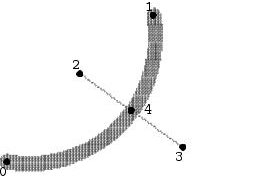
\includegraphics{rightangle.jpg}}
\answerline{}
\answerline{The resulting curve.}
\answerline{\noexpand\end{center}}
\answerline{}
\answerline{Let's sum up by giving together the two instructions solution of this exercise:}
\answerline{}
\answerline{\noexpand\begin{quote}}
\answerline{{\noexpand\tt z4 = .5[z2, z3];}}
\answerline{}
\answerline{{\noexpand\tt draw z0..\char"7B dir(angle(z3 - z2) + 90)\char"7Dz4..z1;}}
\answerline{\noexpand\end{quote}}
\answerline{}
\end{exercise}

So, now you can control the shape of your curves, but you are still limited by the fact that
whatever you do, your curves will always be open. Even when you make the curve end at the point
where it began, like in figure (d), the resulting curve will usually not
be smooth at that point. That's because \MF\ doesn't care if it goes more than once through the
same point. Each time it will be treated independently from the other times. So how do you do to
draw an O, or an 8, or for that matter any closed shape?

Well, your first idea, based on what we've seen until now, could be to fix the direction the
curve has to take on the point where the curve starts end ends (i.e. force the same direction on
starting and ending). For instance, taking again the example of figure
(d), if you write:

\begin{quote}
\begin{verbatim}
draw z0{right}..z5..z4..z2..{right}z0;
\end{verbatim}
\end{quote}

\noindent you will end up with a curve which \emph{looks} smooth and closed (see the figures
for the result of that \texttt{draw} command). The problem with this
approach is that it \emph{obliges} you to control the direction of the curve at its starting
point, something that you may not want to do (you may not even know how to describe the direction
the curve should take). You could always, by a process of trial and error, find the right angle
and use ``\texttt{dir}'', but this would be bad programming, especially since if you decided to
change the position of some points of the curve, you would probably have to change the angle you
chose, again through trial and error. Not much meta-ness in this! Of course you could
always calculate that direction, but this would often ask you for a lot of work, and sometimes it
would just be impossible to do.\footnote{Moreover, \MF\ would still treat the curve as open, even
if it \emph{looks} closed. \MF\ doesn't care what the curve looks like. It considers a curve with
a starting point and an ending point as open, even if those two points are the same. For now, you
needn't care about it, but at a later time you may learn that it's important to know what \MF\ 
considers open and closed.}

\begin{center}
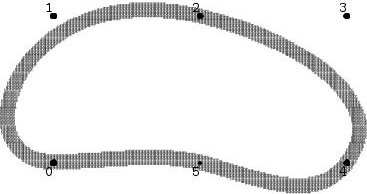
\includegraphics{closedlooking.jpg}\\
The resulting closed-looking curve.
\end{center}

OK, so I've been thoroughly explaining why the previous approach is wrong and impractical, but
I've not yet given an alternative. How on earth are we going to make closed curves then?! Well,
\MF\ has a simple way to do that. Instead of mentioning twice the same point, at the beginning
and the end of the \texttt{draw} command, replace the last mention with ``\texttt{cycle}''. The
presence of this word will tell \MF\ that we want to draw a closed curve, and it will
automatically connect the last point mentioned before ``\texttt{cycle}'' with the first point of
the curve, and in a smooth way.\footnote{And \MF\ will internally treat the curve as closed.} So
if we take our example again, we will write:

\begin{quote}
\begin{verbatim}
draw z0..z5..z4..z2..cycle;
\end{verbatim}
\end{quote}

\noindent and we will get the shape you can see on the closed figure. It is
quite different from the shape on apparently closed figure, because you let \MF\ 
decide the direction the curve would take at point 0, and since there was a symmetry in the
positions of the points describing the curve, it drew it according to this symmetry.

\begin{center}
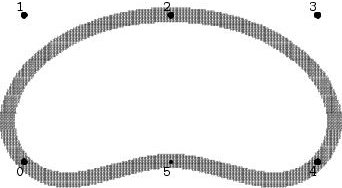
\includegraphics{reallyclosed.jpg}\\
The curve, as drawn using ``\texttt{cycle}''.
\end{center}

\begin{exercise}
Use everything you have learned in this section to write a program which draws a vertical \emph%
{closed} 8 shape. The only conditions are that the shape must be 200 pixels high and that you
must try to use as few points as possible to define your curve.

\answerhead
\answerline{Check out earlier figure, as it nearly gives away a solution to this exercise.}
\answerline{Indeed, if you take points 0 and 3 of that figure and bring them together just under
the two other points, the loop you have would close and look like an 8 shape.}
\answerline{This means that you can define your curve with only three points: the bottom point,
the middle point (where the curve crosses itself) and the top point.}
\answerline{They have the same {\noexpand\tt x} coordinate (since they are vertically aligned),
so you can just put it at 0 for simplicity:}
\answerline{}
\answerline{\noexpand\begin{quote}}
\answerline{{\noexpand\tt x0 = x1 = x2 = 0;}}
\answerline{\noexpand\end{quote}}
\answerline{}
\answerline{\noexpand\noindent (don't forget that you can define the two coordinates of a point
separately).}
\answerline{As for the {\noexpand\tt y} coordinate, let's make the whole thing symmetric and put
point 1 at the middle between point 0 and point 2:}
\answerline{}
\answerline{\noexpand\begin{quote}}
\answerline{{\noexpand\tt y0 = y2 - 200 = 0;}}
\answerline{}
\answerline{{\noexpand\tt y1 = .5[y0, y2];}}
\answerline{\noexpand\end{quote}}
\answerline{}
\answerline{\noexpand\noindent Of course, this is only one way to define the point coordinates,
and you could simply have defined them more directly than I did.}
\answerline{}
\answerline{Now comes the drawing instruction.}
\answerline{Since we want a closed curve, we know that it will end in ``{\noexpand\tt ..cycle}''.}
\answerline{And since we want the curve to cross itself at point 1, we will refer to
{\noexpand\tt z1} twice in the instruction.}
\answerline{You might be tempted to write simply: ``{\noexpand\tt draw z0..z1..z2..z1..cycle;}''.}
\answerline{Unfortunately, the shape that would result from this instruction would only vaguely
look like an 8 shape, and looking at it closely you would realize that it actually doesn't cross
itself at all (try it if you don't believe me), merely comes in contact with itself at point 1.}
\answerline{So how can we ensure that the curve actually crosses itself?}
\answerline{Simply, by specifying the direction it takes at points 0 and 2.}
\answerline{Indeed, if we force the curve to run from left to right (by giving it the
``{\noexpand\tt\char"7B right\char"7D}'' direction) both at points 0 and 2 (or from right to
left, as long as both points receive the same direction), you will oblige the curve to cross
itself, as it's the only way for it to obey the slopes you imposed (try it yourself on a piece of paper.}
\answerline{If you force yourself to draw a closed shape through two points vertically aligned
while going from left to right at both points, the only way to do it is to make an 8 shape).}
\answerline{So the correct drawing instruction is:}
\answerline{}
\answerline{\noexpand\begin{quote}}
\answerline{{\noexpand\tt draw z0\char"7B right\char"7D..z1..z2\char"2B
right\char"7D..z1..cycle;}}
\answerline{\noexpand\end{quote}}
\answerline{}
\answerline{\noexpand\noindent And you can see the result on the figure.}
\answerline{}
\answerline{\noexpand\begin{center}}
\answerline{\noexpand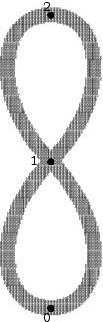
\includegraphics{eightshape.jpg}}
\answerline{}
\answerline{The resulting 8 shape.}
\answerline{\noexpand\end{center}}
\answerline{}
\answerline{But wait a second!}
\answerline{According to the previous paragraph, specifying the same direction on the bottom and
top point should be enough to force the curve to take an 8-like shape.}
\answerline{The middle point shouldn't be necessary at all!}
\answerline{So what would happen if we didn't mention the point 1 in the drawing instruction,
i.e. if we wrote instead:}
\answerline{}
\answerline{\noexpand\begin{quote}}
\answerline{{\noexpand\tt draw z0\char"7B right\char"7D..z2\char"7B right\char"7D..cycle;}}
\answerline{\noexpand\end{quote}}
\answerline{}
\answerline{\noexpand\noindent You can see the result of that instruction on the figure below.}
\answerline{This is indeed a curve which crosses itself exactly at the middle between the
definition points, but its shape is a little less 8-like, and it looks a little like a sandglass.}
\answerline{Why the presence or absence of the middle point in the drawing instruction results in
such different curves is a complicated matter which has to do with the mathematical definition of
the curves as they are handled by \noexpand\MF.}
\answerline{You needn't really worry about it.}
\answerline{Just remember that \noexpand\MF's idea of the ``best'' curve following your
instructions is not always what you expect, and that \noexpand\MF\ is {\noexpand\it very}
sensitive to the curve definitions you give.}
\answerline{}
\answerline{\noexpand\begin{center}}
\answerline{\noexpand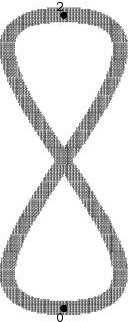
\includegraphics{sandglassshape.jpg}}
\answerline{}
\answerline{A sandglass-looking shape.}
\answerline{\noexpand\end{center}}
\answerline{}
\answerline{In any case, the 2-point solution to this exercise was not necessary to pass it.}
\answerline{If you found its 3-point solution, you have correctly solved the exercise already.}
\end{exercise}

\section{Pens}
\label{lesson2:pens}

If you have been curious enough to try and reproduce some of the figures you've seen until now,
you must have noted that your results, while correct in shape, are slightly different from some
of what have seen in this tutorial. Namely, the curves you have produced are thicker. For
instance, if you tried to reproduce the closed shape in the earlier figure, what you have
obtained was probably closer to the next figure. And you have been
especially unable to reproduce the figures using thin lines that are present in this tutorial.
Yet I have produced all those figures with \MF\ exclusively. So what have I done to get lines of
a different thickness from what you get?

\begin{center}
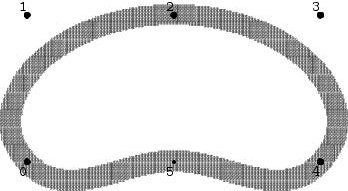
\includegraphics{closedthick.jpg}\\
A thick closed curve.
\end{center}

If you know a little about how computers work, and especially how they do graphics, you probably
have realized that the way I've been explaining how \MF\ handles graphics is a metaphor, namely
the metaphor of \emph{drawing}. Indeed, \MF\ is not a man behind a desk with a sheet of paper in
front of him. It's a program, and all it does when handling graphics is handle a grid of pixels,
small units of space which have only two states: white or black. And what \MF\ does is tell which
pixels are black and which ones stay white. However, the metaphor of drawing is very useful,
because from our perspective it looks \emph{exactly} as if \MF\ was actually a man behind a desk
drawing on a piece of paper what we order him to draw. It's not for nothing that the main drawing
instruction is called \texttt{draw}. For instance, just as when we are drawing by hand,
\MF's curves behave just as if they are drawn in a certain sense, from one point to the other
(the order being of course the order of the points as given behind the \texttt{draw}
instruction). This explains why adding a direction as a vector between braces works as we expect
it, and why giving an opposite sense can modify a curve so strongly (just check again
left and right figures), and exactly the same way as it would do if you draw
the curve yourself by hand.

But this metaphor of drawing can be further extended. Indeed, when you want to draw something,
you need not only your hand and a piece of paper, but also a \emph{pen}, without which you could
never mark anything on the paper! And depending on the kind of pen you're using (a pencil, a
ballpoint pen, a fountain pen, or one of those fancy calligraphic pens with special tips), you
will get different results, even if the shape you draw is always the same. Well, in \MF\ you just
do exactly the same! \MF\ has a command called \texttt{pickup} that allows you to choose the pen
it will use to draw the curves you ask it to draw with the \texttt{draw} command. By using it,
you can specify a pen whose tip is more or less big, more or less circular (or of some other
shape) etc. The \texttt{pickup} command must simply be followed by the name of the pen you
want to use.

But to choose a pen, you need pens to choose from! Well, it's no problem, because \MF\ has a few
predefined pens ready for use, besides the default pen that it automatically uses when you don't
pick up another one, and that you've been using until now. The two main predefined pens, that you
will mostly use, are called \texttt{pencircle} and \texttt{pensquare}. They correspond
respectively to a pen whose tip is a circle of 1 pixel of diameter and a pen whose tip is a
square of side 1 pixel. Check out circle and square pen figures to see a familiar
shape drawn this time using those very thin pens. They were drawn by adding respectively
``\texttt{pickup pencircle};'' and ``\texttt{pickup pensquare};'' in front
of the actual drawing instruction.

\begin{center}
\begin{tabular}{ccc}
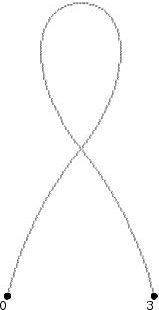
\includegraphics{circleloop.jpg} & \hspace{2cm} & 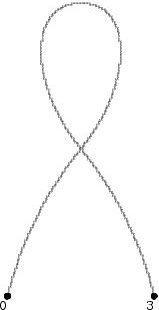
\includegraphics{squareloop.jpg} \\
(a) & & (b) \\
\end{tabular}\\
The same loop as before, but drawn with (a) \texttt{pencircle} and (b) \texttt{pensquare}.
\end{center}

Now, for how useful tiny pens can be, what we want usually is bigger pens, i.e. pens with a
bigger tip, like the ones I've been using myself. But how can you get such pens when all you have
is pens with very small tips? The answer is actually quite simple: \emph{transform} them! Yes,
you understood correctly. All those transformations that we briefly mentioned earlier
can apply not only to pair values, but also to pens! Or at least, the
transformations that are meaningful in this situation can be applied here. Indeed, since our goal
is to change the shape and/or size of our pens, a transformation like ``\texttt{shifted}'',
``\texttt{rotatedaround}'' or ``\texttt{reflectedabout}'' is useless. However, ``\texttt%
{scaled}'' (to change the global size of our pentip), ``\texttt{xscaled}'' and ``\texttt%
{yscaled}'' (to stretch our pentip on one direction only) can be usefully used with pens. For
instance, by specifying:

\begin{quote}
\begin{verbatim}
pickup pencircle scaled 10;
\end{verbatim}
\end{quote}

\noindent you create a pen whose tip is a circle of 10 pixels of diameter. If you write:

\begin{quote}
\begin{verbatim}
pickup pensquare xscaled} 20;
\end{verbatim}
\end{quote}

\noindent you will obtain a pen with a rectangular tip 20 pixels wide and 1 pixel tall. And you
can of course concatenate transformations, like in:

\begin{quote}
\begin{verbatim}
pickup pencircle xscaled 10 yscaled 35;
\end{verbatim}
\end{quote}

\noindent which makes subsequent drawing done with a pen whose tip is ellipsoidal, with a
horizontal axis 10 pixels long and a vertical axis 35 pixels long. Check out the flatpen figures
to see how different pens can really change how otherwise identical curves
look like.

\begin{center}
\begin{tabular}{cc}
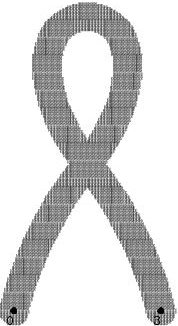
\includegraphics{flatpen1.jpg} &
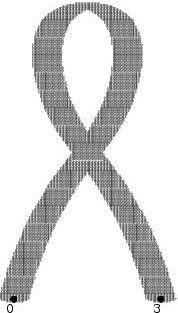
\includegraphics{flatpen2.jpg} \\
\texttt{pencircle scaled 20;} &
\texttt{pencircle xscaled 20 yscaled 5;} \\
(a) & (b) \\
\end{tabular}

\begin{tabular}{cc}
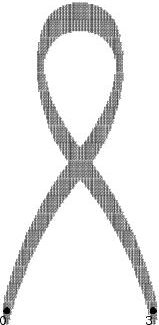
\includegraphics{flatpen3.jpg} &
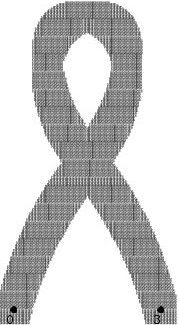
\includegraphics{flatpen4.jpg} \\
\texttt{pencircle xscaled 5 yscaled 20;} &
\texttt{pensquare scaled 20;} \\
(c) & (d) \\
\end{tabular}

\begin{tabular}{cc}
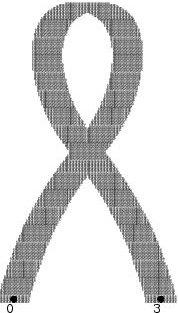
\includegraphics{flatpen5.jpg} &
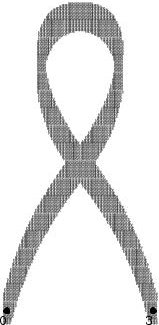
\includegraphics{flatpen6.jpg} \\
\texttt{pensquare xscaled 20 yscaled 5;} &
\texttt{pensquare xscaled 5 yscaled 20;} \\
(e) & (f) \\ 
\end{tabular}\\
Examples of the same loop drawn with different pens.
\end{center}

\begin{exercise}
List at least three different ways to pick up a 5-pixel-high, 20-pixel-wide, ellipsoidal pen.

\answerhead
\answerline{The most obvious way to pick up such a pen is of course to use the ``{\noexpand\tt
xscaled}'' and ``{\noexpand\tt yscaled}'' transformations with a {\noexpand\tt pencircle}, as
such:}
\answerline{}
\answerline{\noexpand\begin{quote}}
\answerline{{\noexpand\tt pickup pencircle xscaled 20 yscaled 5;}}
\answerline{\noexpand\end{quote}}
\answerline{}
\answerline{\noexpand\noindent It is the easiest (and most advisable) way to do it, but certainly
not the only one!}
\answerline{Indeed, you can also use ``{\noexpand\tt scaled}'' itself together with a combination
of ``{\noexpand\tt xscaled}'' and ``{\noexpand\tt yscaled}'' to obtain the same result.}
\answerline{For instance, since the smallest dimension of the wanted pen is 5 pixels, you can
first scale {\noexpand\tt pencircle} by 5, and then stretch it horizontally by a factor of 4 to
obtain the wanted ellipsoidal pen:}
\answerline{}
\answerline{\noexpand\begin{quote}}
\answerline{{\noexpand\tt pickup pencircle scaled 5 xscaled 4;}}
\answerline{\noexpand\end{quote}}
\answerline{}
\answerline{\noexpand\noindent You can also scale it first by the biggest dimension (here 20) and
then {\noexpand\it shrink} it vertically by scaling with a fractional factor:}
\answerline{}
\answerline{\noexpand\begin{quote}}
\answerline{{\noexpand\tt pickup pencircle scaled 20 yscaled .25;}}
\answerline{\noexpand\end{quote}}
\answerline{}
\answerline{\noexpand\noindent You could even go wild and make something strange like:}
\answerline{}
\answerline{\noexpand\begin{quote}}
\answerline{{\noexpand\tt pickup pencircle scaled 56 xscaled 5/14;}}
\answerline{\noexpand\end{quote}}
\answerline{}
\answerline{\noexpand\noindent Go ahead, make the calculations, and you'll see that it does
create a 5-pixel-high, 20-pixel-wide pen.}
\answerline{Depending on the factor you first put with ``{\noexpand\tt scaled}'', you actually have an
infinity of possibilities which all result in the wanted pen.}
\answerline{But if you find them silly, don't worry: you're not the only one!}
\answerline{The first three propositions were the only ones necessary to correctly solve this exercise.}
\end{exercise}

However, if all you can do is scaling \texttt{pencircle} and \texttt{pensquare}, you'll rapidly
be limited in what you can do. Even when scaling with different factors horizontally and
vertically, all you can get is horizontal or vertical pens. And if you know a little about
calligraphy, you know that what influences most the looks of letters, besides the shapes of the
curves, is the position of the thin and thick strokes. And what fixes their positions is the
\emph{angle} the pen nib makes with horizontality. Calligraphers will turn their pens differently
depending on the result they want to achieve. And it's something \MF\ can easily do by \emph%
{rotating} its pens. Indeed, although the ``\texttt{rotatedaround}'' transformation cannot be
used with pens, the ``\texttt{rotated}'' transformation can, and has the expected effect of
putting the pen nib at an angle with horizontality. The next figure shows the
effect the angle alone of a pen can have on the looks of otherwise identical curves.

\begin{center}
\begin{tabular}{cc}
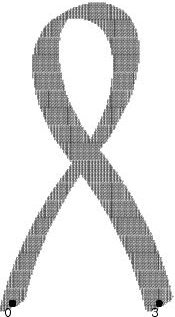
\includegraphics{anglepen1.jpg} &
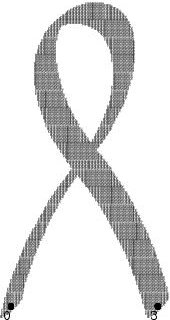
\includegraphics{anglepen2.jpg} \\
\texttt{pencircle xscaled 20} &
\texttt{pencircle xscaled 20} \\
\texttt{yscaled 5 rotated 30;} &
\texttt{yscaled 5 rotated 45;}\\
(a) & (b) \\
\end{tabular}

\begin{tabular}{cc}
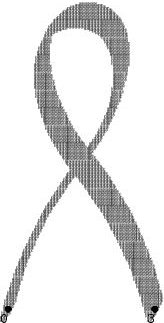
\includegraphics{anglepen3.jpg} &
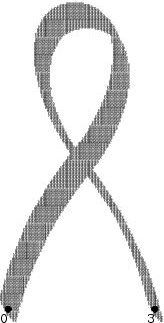
\includegraphics{anglepen4.jpg} \\
\texttt{pencircle xscaled 20} &
\texttt{pencircle xscaled 20} \\
\texttt{yscaled 5 rotated 60;} &
\texttt{yscaled 5 rotated 120;}\\
(c) & (d) \\
\end{tabular}

\begin{tabular}{cc}
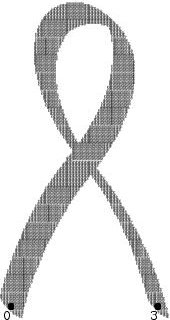
\includegraphics{anglepen5.jpg} &
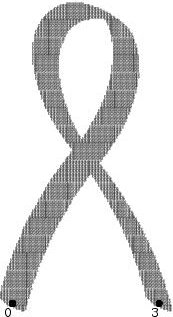
\includegraphics{anglepen6.jpg} \\
\texttt{pencircle xscaled 20} &
\texttt{pencircle xscaled 20} \\
\texttt{yscaled 5 rotated 135;} &
\texttt{yscaled 5 rotated 150;} \\
(e) & (f) \\ 
\end{tabular}\\
Again the same loop drawn with pens of identical shape but tilted at different angles.
\end{center}

\begin{exercise}
Imagine that you want to pick up a rectangular pen 20 pixels wide and 2 pixels high (a very thin
pen thus). However, you want it tilted, so that its longest side will be perpendicular to the
direction defined by two points 1 and 2. Note that we don't give any condition on the positions
of those two points, only that they have already been defined before you pick up the pen. How
would you solve this problem?

\answerhead
\answerline{Defining a rectangular 20-pixel-wide 2-pixel high pen is easy.}
\answerline{ The line ``{\noexpand\tt pensquare xscaled 20 yscaled 2}'' solves that problem.}
\answerline{However, you still have to add a ``{\noexpand\tt rotated}'' transformation to finish
the job.}
\answerline{But how do we find the correct angle of rotation?}
\answerline{}
\answerline{This problem is actually trivial if you remember the beginning of this lesson, where
we defined the ``{\noexpand\tt angle}'' operator.}
\answerline{Remember also that when you have two points labeled 1 and 2, the quantity
{\noexpand\tt z2 - z1} is a vector whose direction is the one defined by the two points, and that
for this reason ``{\noexpand\tt angle(z2 - z1)}'' is the angle this direction makes with
horizontality.}
\answerline{And in order to have your pen perpendicular to that direction, you just need to
rotate it by that angle plus 90$^\circ$.}
\answerline{So you finally pick up the correct pen through the following command:}
\answerline{}
\answerline{\noexpand\begin{quote}}
\answerline{{\noexpand\tt pickup pensquare xscaled 20 yscaled 2 rotated (angle(z2 - z1) + 90);}}
\answerline{\noexpand\end{quote}}
\answerline{}
\answerline{\noexpand\noindent Note the use of parentheses to make sure that the addition is
correctly interpreted.}
\end{exercise}

\section{Once more, with character!}

Now I want you to play a bit with your newly acquired knowledge.

\begin{exercise}
Go back the the last capital letter E you made and make some new files: \texttt{e045.mp},
\texttt{e015.mp}, $\ldots$
Make a series of capital Es with an ellipsoid pen, \texttt{xscaled} by $20$ and \texttt{yscaled}
by $2$.
Then I want you to try every 45$^\circ$ rotation possible from 0$^\circ$ to 315$^\circ$ and just
see what the results look like.
\end{exercise}

\chapter{Simple Fonts / Alphabets / Ideographs}

For almost the rest of these lessons we are going to visit with a variety of writing types and
try making a few glyphs and getting them to work in \TeX.
My hope is to both go from simple systems to complicated systems, but at the same time provide
enough information that you can make any writing system you want.

Each of these lessons will have a similar structure.

\begin{itemize}
\item \textbf{Introduction} --- a brief explanation of what we hope to accomplish.
The names of the lessons are not always strictly correct and this will correct some of that.
\item \textbf{Language} --- a list of the glyphs we want to make.
None of these will be a full language, just enough to get you pointed in the right direction.
\item \textbf{Glyphs} --- the actual work of drawing the glyphs we want.
\item \textbf{Extras} --- either extra things we need to happen in order to get this system to
work correctly or sometimes just bonus material that I think might be fascinating.
\end{itemize}

\section{Introduction}

This lesson is covering what is sometimes called a \emph{simple orthography}, that is a system of
writing with unique and separated glyphs.
Examples of such a system are the Roman Alphabet, the syllabaries of Ethiopian and Cherokee, the
glyphs of Chinese, and even the mixed syllabaries and glyphs of Japanese.
What each of these systems have in common is that you can encode them as a simple system of one
glyph to one number.
If you had a keyboard, you could place one symbol on each key and the user could reasonably
expect that the machine would make that image and move forward one space to be ready for the next
one.
In this lesson, the difference between writing in English and writing in Chinese is a question of
quantity, not complexity.
By default we only have support for up to 256 individual glyphs, so if you do want to support a
system like Chinese using only material from this lesson then you will need to make multiple
fonts in \MF\ and switch between those fonts in \TeX.

\section{Language}

Our language will consist of one character in two locations.
The A letter of the \textit{Moon Alphabet}, also called \textsl{The Moon System of Embossed Reading}.

\section{Glyphs}

In some respects you have already done this work.
At least, you have if you did all those exercises regarding the capital letter E.
I eventually settled on this.

\begin{quote}
\tt
z1=(0,0); z2=(5,60); z3=(25,100); z4=(45,60); z5=(50,0);\\
draw z1--z2{up}..z3..{down}z4--z5;
\end{quote}

But that's not really fair.
So let's talk about experimenting.

If you don't have a display, then what you have to do is create a series of very similar files.
For instance: \texttt{z2=(5,60);} in one and \texttt{z2=(10,60);} in another and so forth.
Then set up a script to run them all and compare the results.

If you do have a display, then you need to try the \texttt{clearit;} command.
This is how I actually came up with this.
I started up \MF, entered \verb|\relax|, typed in \texttt{1+1;} and told it to be in nonstop
and then was ready when I typed in \texttt{showit;}.
My first experiment was:

\begin{quote}
\tt
draw (0,0)..(25,100)..(50,0); showit;
\end{quote}

After this I started experimenting with this line.

\begin{quote}
{\tt\small
clearit; draw (0,0)\{dir 0\}..(25,100)..\{dir 180\}(50,0); showit;\\
clearit; draw (0,0)\{dir 10\}..(25,100)..\{dir 170\}(50,0); showit;\\
clearit; draw (0,0)\{dir 20\}..(25,100)..\{dir 160\}(50,0); showit;\\
}
$\cdots$
\end{quote}

When I couldn't get that to pan out I started experimenting with two additional points, and
finally added in the directions and line segments.

It's not meta.
There has been no attempt to mention that \texttt{y1} is the same as \texttt{y5} or that
\texttt{x3} is half way between \texttt{x1} and \texttt{x5}.
But more importantly, that doesn't matter.

Personally, I don't want to add meta-ness when I come back and finesse my fonts.
Until I have a fairly full font, I don't have any idea what the meta-ness \emph{should} be.
For this particular font, \texttt{y1} should equal \texttt{y5} but what will probably turn out
being more \emph{important} is that \texttt{y1} \textbf{and} \texttt{y5} are equal to a
\texttt{baseline} parameter.
So it's not that I'm against meta-ness, I just don't want to pre-emptively add it too early when
I'm still experimenting with shapes and ideas.
Maybe my first experiments will have a baseline, maybe I will decide later that they hang down
from a topline instead and my \texttt{y1} and \texttt{y5} will be different but \texttt{y3} will
use the \texttt{baseline} parameter.

There is also most likely better ways to get this shape or even make it better.
But I'm \textsc{ok} with that, because I'm still experimenting.
I got a great picture that I'm happy with, but how do we turn this into an actual font?

\begin{verbatim}
MOON_LETTER_A = 65; % hex "0041";
MOON_LETTER_a = 97; % hex "0061";

u#:=20/36pt#;           % unit width
cap_height#:=246/36pt#; % height of caps
define_pixels(u);

vardef draw_moon_letter_a =
    z1=( 0u+1u,0.0h);
    z2=( 1u+1u,0.6h);
    z3=( 5u+1u,   h);
    z4=( 9u+1u,0.6h);
    z5=(10u+1u,0.0h);
    pickup pencircle scaled 10;
    draw z1--z2{up}..z3..{down}z4--z5;
    labels(range 1 thru 5);
enddef;

beginchar(MOON_LETTER_A,12u#,cap_height#,0);
    draw_moon_letter_a;
endchar;

beginchar(MOON_LETTER_a,12u#,cap_height#,0);
    draw_moon_letter_a;
endchar;

end;
\end{verbatim}

Our first two lines (\texttt{MOON\_}) define the values we want these characters to be associated
with.

The next section \texttt{u\#:=} defines some values that we will be using.
The value \texttt{u} feels like about $1/10$th of of the width of the character --- primarily
because that's what I will define it as later.
If I'm being completely honest, I chose \texttt{20/36pt} because I see that a lot in Computer
Modern --- read \textsl{The \MF Book} for more.
The \texttt{cap\_height} the the height of capital letters.
And \texttt{define\_pixels} is required my \MF.

The \texttt{vardef} section is where I define a section I am using more than once.
You will notice that I have horizontally spaced out the \texttt{z} definitions.
That's just because it's the way I like it.
I have also adjusted for the character width so what used to be \texttt{z2=(5,60);} for a
character 50 wide and 100 tall has become \texttt{1u,0.6h);}.
You could also use something like this to make a cuneiform font if you wanted.

Then I define the two characters for my font --- uppercase A and lowercase a.
When we look at \texttt{beginchar(MOON\_LETTER\_A,12u\#,cap\_height\#,0);}:\\
\phantom{\hskip 1 cm}\texttt{MOON\_LETTER\_A} is the character code we want to assign this glyph
to.\\
\phantom{\hskip 1 cm}\texttt{12u\#} is how wide we want the character to be.
In my case, that's 12 units of horizontal space (the $1/10$th I mentioned earlier) plus an
$1/10$th on each side.\\
\phantom{\hskip 1 cm}\texttt{cap\_height\#} is the height of capital letters.\\
\phantom{\hskip 1 cm}The final \texttt{0} is how far below the baseline any tail drops.\\
The call to the function would normally consist of unique commands, but I wanted to show this
option as well.

Finally I tell \MF\ I am done with \texttt{end;}.
In actuality \MF\ only needs to see \texttt{end} and never notices the trailing \texttt{;}, but
it always looks funny to me without it.

Now that we have this let's take a look at our beautiful font.

\begin{quote}
\begin{verbatim}
mf moon.mf
gftodvi moon.2602gf
dvipdf moon.dvi
\end{verbatim}
\end{quote}

This should give you a two page \texttt{pdf} file and both pages should look suspiciously similar.
Now let's turn this into a font.

\begin{quote}
\begin{verbatim}
mf '\mode=ljfour; mode_setup; input moon.mf'
gftopk moon.600gf
\end{verbatim}
\end{quote}

And now let's try it out.
Create a \LaTeX\ file with the following lines and see what comes from it.

\begin{quote}
\begin{verbatim}
\documentclass{article}

\begin{document}
\newfont{\moon}{moon}

{\moon
A a
}
\end{document}
\end{verbatim}
\end{quote}

When you take a look at it, you'll notice that there is no space between these two letters.
That is correct, we did not define the space character in this font!
Though perhaps your language does not have spaces yet you want to include spaces in your sources
as a convenience to yourself.

\section{Extras}

For this first writing type I want to mention some additional pen choices and how to organize
files.

\subsection{Pens}

I didn't play with any pens but, again, that's something I would want to play with later when I
have a better sense of the writing as a whole.
If you want to have some idea of really good calligraphic features that align nicely with what
you have learned in this tutorial, check out the script font by K.~U.~Leuven.
If your distribution doesn't have it check out \texttt{http://ctan.org/tex-archive/fonts/script}.

If you study Computer Modern you will find that they do not do this.
Why?
In the case of Computer Modern, the font was already well understood and had needs well beyond
simulating pens.
Even so, there is one additional technique I want to quickly demonstrate.

Use \MF\ to try out the following one step at a time with a \texttt{clearit;} before and a
\texttt{showit;} afterwards.
If you are really feeling adventurous, try turning these progressive experiments into the letters
B, C, D, and E.

\textbf{Experiment 1:}
Our current state.

\begin{quote}
\begin{verbatim}
draw (0,0)..(0,75)..(25,100)..(25,0)..cycle;
\end{verbatim}
\end{quote}

\noindent
Perhaps not a very useful (or even beautiful) shape, but exactly the type of thing we are used
to.

\textbf{Experiment 2:}
As thin as can be.

\begin{quote}
\begin{verbatim}
pickup pencircle scaled 0;
draw (0,0)..(0,75)..(25,100)..(25,0)..cycle;
\end{verbatim}
\end{quote}

\noindent
Hopefully no surprises here.

\textbf{Experiment 3:}
A new command.

\begin{quote}
\begin{verbatim}
pickup pencircle scaled 0;
fill (0,0)..(0,75)..(25,100)..(25,0)..cycle;
\end{verbatim}
\end{quote}

\noindent
This is much more akin to how modern font tools work.
If you have played with FontForge you will see that you make outlines and fill them in.
Though we can now use this to make letters like capital E, we can't make letters like capital A
with this technique.

\textbf{Experiment 4:}
Another new command.

\begin{quote}
\begin{verbatim}
pickup pencircle scaled 0;
fill (0,0)..(0,75)..(25,100)..(25,0)..cycle;
unfill (10,10)..(10,65)..(15,80)..(15,10)..cycle;
\end{verbatim}
\end{quote}

\noindent
Now we can use this to make any letter.
I've never personally tried this technique to make a letter.
If you decide to move from a pen-based writing system to something more like a printing press
then this may be a way to go.
It will allow for all sorts of letter decorations (like serifs) to be attached which may exist
but not be a part of general penmanship.

\subsection{Organizing files}

Keeping everything in one master file can quickly get files to be unwieldy.
You should give some early thoughts to dividing your work up.
Let's see how Computer Modern does this.

First, take a look at \texttt{cmr10.mf} and you will find an attempt to \texttt{input cmbase},
After that are a set of parameters, the meta-ness of Computer Modern.
At the end you will see a command to \texttt{generate roman}.
If search through \texttt{cmbase} you will find that \texttt{generate} is an alias for
\texttt{input}.
So what is really happening here is \texttt{roman.mf} is being \texttt{input}.
Taking a look at \texttt{roman.mf} you will find at the beginning:

\begin{quote}
\begin{verbatim}
input romanu;  % upper case (majuscules)
input romanl;  % lower case (minuscules)
input greeku;  % upper case Greek letters
input romand;  % numerals
input romanp;  % ampersand, question marks, currency sign
input romspl;  % lowercase specials (dotless \i, ligature \ae, etc.)
input romspu;  % uppercase specials (\AE, \OE, \O)
input punct;  % punctuation symbols common to roman and italic text
input accent;  % accents common to roman and italic text
if ligs>1: input romlig; fi  % letter ligatures
if ligs>0: input comlig; fi  % ligatures common with italic text
if ligs<=1: input romsub; fi  % substitutes for ligatures
\end{verbatim}
\end{quote}

Here Computer Modern inputs a bunch of files which happen to define things like A--Z, a--z,
numbers, and punctuation.
Then, depending on the setting of \texttt{ligs} which were already set by the \texttt{cmr10.mf}
file (among others) to decide what to put in other non-standard locations.

If you take a look at \texttt{romanu.mf}, you will find all the letters defined in order.
If you know what you will be making, that's not a bad way to go.
I might take it one step further and have \texttt{romanu.mf} set some variable and
\texttt{input} the letters in order.
I imagine something like

\begin{quote}
\begin{verbatim}
current_char_code := current_char_code + 1; input roman_letter_a;
\end{verbatim}
\end{quote}

\noindent
which let's me quickly move them around as I play with the order they should be in or change my
mind about transliteration.

Actually, I might skip the middle level and have \texttt{cmr10.mf} do the \texttt{input} the
letters in order especially since this will help as we try to turn our \MF\ fonts into a modern
font.
On the other hand the middle layer does let you know that the letters are in the same order in
every font.
Regardless, it's something to think about.

\chapter{Accents and Abjads}

In this lesson I hope to teach you enough about accents that you can add one (or two) accents to
any letter you choose.

\section{Introduction}

There's actually a few things to introduce here.

\subsection{Abjads}

Strictly speaking, \textbf{abjad}s do not need accents of any kind.
In an pure abjad, the techniques of alphabets in the prior lesson would work just fine.
There would be one symbol per consonant and enough context to determine the vowels.
But there are many abjads which are not pure and, for reasons not well understood, these writing
systems seem to like to add these vowels by means of small accent marks.
Sometimes for all of them but often only for the surprising vowel sounds.

\subsection{What are accents}

Abjad users aren't the only ones.
Whenever I spell \emph{co\"ordinate}, I am using an accent that tells you that this word does not
follow the normal rules of pronounciation.
That \"\ says that it begins with a /c\=o$\cdot$\=ord/ and not /c\t oord/.

Sometimes the accents are so integrated that they are considered new letters, our J used to be I
an extended tail.

Other times what looks like an accent is just part of the letter: we have i and j but not \i\ nor
\j.

What really determines whether something is an accent or not is how the users of the system treat
them.
If they see them as separate letters, then they are separate letters even if they write it as a
base letter plus an accent mark.

\subsection{Typing accents}

There are about three different methods for handling accents.

First, you can treat it as a separate letter anyway and just go for it.
Some digital fonts (and keyboard drivers) have done this even when the language considers it an
accent.

Second, you can take what's called the \textbf{dead-key} approach.
There are special \emph{accent keys} which do nothing when pressed --- they are dead keys.
When you type the next key, if it can accept that accent, then it is accented.
If it can't accept that accent, then it just types normally.
\TeX\ and \MF\ (as well as many keyboard drivers) do this.
When I want to say \"o\ in \TeX\ I have to type \verb|\"o| which is effectively a \texttt{"} dead
key followed by a compatible base character.

Third, you can take what's called the \textbf{combining} approach.
There are special \emph{accent keys} which go back and add an accent to the prior character.
This is what \textsc{Unicode} (and modern digital fonts) do.
So even if you type using a dead key approach, the computer may be switching things around for
you.

This means that for this lesson, you won't be learning about how \TeX\ and \MF\ handle accents.
You will instead be learning how to make accents that will evenutually work nicely with modern
digital fonts.

\subsection{Limits}

Even though many abjads are right to left writing, we won't be covering that yet.
And we won't be talking about writing systems like Arabic that change form depending on the
letters around them.
We are just talking about adding accents.

In order to make accents look as good as possible, you really need to custom make all the glyphs
you want to support with individual accent marks.
Doing this is more a question of either kerning or ligatures (and a future lesson).
We are taking the simple approach for now which should let you get something up and running.

\section{Language}

Our language will consist of one letter and three accents.
The base letter will look quite a bit like our letter o.
The accents will be a hat above the o, a pair of dots within the o, and a curve below the o.

\section{Glyphs}

We've talked about thinking through orgainizing files before we get too involved.
Let's actually do that this time.

\begin{quote}
\begin{tabular}{lcl}
\texttt{ofont.mf}     &---&The entire font.\\
\texttt{ochar.mf}     &---&Our base character.\\
\texttt{accenthigh.mf}&---&The high accent.\\
\texttt{accentmid.mf} &---&The middle accent.\\
\texttt{accentlow.mf} &---&The low accent.\\
\end{tabular}
\end{quote}

Let's take a look at our primary font file first.
The file \texttt{ofont.mf} looks like this:

\begin{quote}
\begin{verbatim}
u#:=20/36pt#;           % unit width
cap_height#:=246/36pt#; % height of caps
define_pixels(u);

char_code:= hex "0040";

char_code:=char_code+1; input ochar;

char_code:= hex "0060";

char_code:=char_code+1; input accenthigh;
char_code:=char_code+1; input accentmid;
char_code:=char_code+1; input accentlow;

end;
\end{verbatim}
\end{quote}

So this is exactly as I explained.
If I change my mind about the proper order of the accents, I just have to move them around.
By making the first \texttt{char\_code} start at a value of 64, that means the next letter is in
the place of capital A.
By making the second \texttt{char\_code} start at a value of 96, that means the accents start at
lowercase a.
So much for the primary font file, let's see our base character shape.
The file \texttt{ochar.mf} look like this:

\begin{quote}
\begin{verbatim}
beginchar(char_code,12u#,cap_height#,0);
    z1=( 5u+1u,0.0h);
    z2=( 0u+1u,0.4h);
    z3=( 5u+1u,0.8h);
    z4=(10u+1u,0.4h);
    pickup pencircle scaled 5;
    draw z1..z2..z3..z4..cycle;
    labels(range 1 thru 5);
endchar;
\end{verbatim}
\end{quote}

Absolutely none of this should come as a surprise.
Now let's go see our first accent mark.
If we take a look at \texttt{accenthigh.mf} we find:

\begin{quote}
\begin{verbatim}
beginchar(char_code,0u#,cap_height#,0);
    z1=(3u-11u,0.9h);
    z2=(5u-11u,   h);
    z3=(7u-11u,0.9h);
    pickup pencircle scaled 5;
    draw z1--z2--z3;
    labels(range 1 thru 3);
endchar;
\end{verbatim}
\end{quote}

This may not look too unusual at first, but take a closer look at \texttt{beginchar}.
The second argument (the width) is 0!
We have just defined a character that has a width of 0---that is, after this character has been
added to the page then \TeX\ is to not advance any amount before moving onto the next character.
This is the reverse of the dead key.
What we have here is a dead character.
So you type ``o'', and \TeX\ moves forward ready for your next character;
then you type \"\ and \TeX\ ignores it when assembling the page--- though ink will still be added
when it is time to paint the page.

Take a second look and notice the co\"ordinate \texttt{z1}.
\texttt{z1=(-8u,0.9h)}.
\MF\ has been instructed to place ink both outside and to the left of the glyph space.
So this accent (of no space) goes back and adds ink to the previous character.
Which should not seem that off since that is what people do as well.

Alright, let's take a look at the two other accent characters and see what they look like.
In \texttt{accentmid.mf} we find:

\begin{quote}
\begin{verbatim}
beginchar(char_code,0u#,cap_height#,0);
    z1=(4u-11u,0.4h);
    z2=(6u-11u,0.4h);
    pickup pencircle scaled 5;
    draw z1;
    draw z2;
    labels(range 1 thru 2);
endchar;
\end{verbatim}
\end{quote}

\noindent And in \texttt{accentlow.mf} we find:

\begin{quote}
\begin{verbatim}
beginchar(char_code,0u#,cap_height#,0);
    z1=(3u-11u,-0.2h);
    z2=(5u-11u,-0.1h);
    z3=(7u-11u,-0.2h);
    pickup pencircle scaled 5;
    draw z1..z2..z3;
    labels(range 1 thru 3);
endchar;
\end{verbatim}
\end{quote}

Now let's build the font.

\begin{quote}
\begin{verbatim}
mf '\mode=ljfour; mode_setup; input ofont.mf'
gftopk ofont.600gf
\end{verbatim}
\end{quote}

And let's test it out.

\begin{quote}
\begin{verbatim}
\documentclass{article}

\begin{document}

\newfont{\ofont}{ofont}

Letter by itself.

{\ofont A }

Letters with one accent.

{\ofont Aa Ab Ac }

Letters with two accents.

{\ofont Aab Aac Abc }

Now one hunderd letters with all three accents!

{\ofont
Aabc Aabc Aabc Aabc Aabc Aabc Aabc Aabc Aabc Aabc
Aabc Aabc Aabc Aabc Aabc Aabc Aabc Aabc Aabc Aabc
Aabc Aabc Aabc Aabc Aabc Aabc Aabc Aabc Aabc Aabc
Aabc Aabc Aabc Aabc Aabc Aabc Aabc Aabc Aabc Aabc
Aabc Aabc Aabc Aabc Aabc Aabc Aabc Aabc Aabc Aabc
Aabc Aabc Aabc Aabc Aabc Aabc Aabc Aabc Aabc Aabc
Aabc Aabc Aabc Aabc Aabc Aabc Aabc Aabc Aabc Aabc
Aabc Aabc Aabc Aabc Aabc Aabc Aabc Aabc Aabc Aabc
Aabc Aabc Aabc Aabc Aabc Aabc Aabc Aabc Aabc Aabc
Aabc Aabc Aabc Aabc Aabc Aabc Aabc Aabc Aabc Aabc
}

\end{document}
\end{verbatim}
\end{quote}

\section{Extras}

This will give you accents, but it also assumes that all the characters are of a similar width.
If you had a character that looked more like an I or l, then these accents would be too far to
the left.
If you had a character that had a width more like an M or W, then the accent would be too far to
the right.

One solution to that is to make every character have the same width.
Another is to have different accents.
The better answer is handled in next lesson.

\chapter{From \MF\ to Modern Fonts}

So it's quite wonderful that we have these fonts that we can use in \TeX, but how do we share
these fonts with others, or even use these fonts in places outside of the world of \TeX?

\section{History}

Remember way back in the preface that I stole from Christophe~Grandsire we talked about the
history of \MF?
Now we are going to talk about the history of \MF\ since then.

In that preface I mentioned in passing that Computer Modern ``served as the base for other font
families like Computer Concrete.''
But Computer Modern wasn't just the base for Computer Concrete.
Thanks to the huge amount of meta-ness in Computer Modern, Computer Concrete was the same font
with different parameters.
Computer Modern was so meta and could be used to make so many fonts that one almost wonders why
anyone ever made any fonts.
Fonts were made, but never to the level that Knuth made his fonts unless someone was extending
Computer Modern to support additional letters.

During the 1980s the personal computer became much more common.
But these early home appliances could not actually run something like \MF\ and/or \TeX.
What they could do is allow someone to make a document that was \emph{nicer} than just using a
using a typewriter.
Digital fonts were created, simple pixel based images that people could make on their own to get
the exact effect they wanted as long as they were willing to make a new font for every device

\immediate\closeout\mfanswers

\appendix

\input{mf4clans.tex}

\chapter{GNU Free Documentation License}
\label{mfgfdl}

 \begin{center}

       Version 1.2, November 2002


 Copyright \copyright 2000,2001,2002  Free Software Foundation, Inc.
 
 \bigskip
 
     59 Temple Place, Suite 330, Boston, MA  02111-1307  USA
  
 \bigskip
 
 Everyone is permitted to copy and distribute verbatim copies
 of this license document, but changing it is not allowed.
\end{center}


\begin{center}
{\bf\large Preamble}
\end{center}

The purpose of this License is to make a manual, textbook, or other
functional and useful document "free" in the sense of freedom: to
assure everyone the effective freedom to copy and redistribute it,
with or without modifying it, either commercially or noncommercially.
Secondarily, this License preserves for the author and publisher a way
to get credit for their work, while not being considered responsible
for modifications made by others.

This License is a kind of "copyleft", which means that derivative
works of the document must themselves be free in the same sense.  It
complements the GNU General Public License, which is a copyleft
license designed for free software.

We have designed this License in order to use it for manuals for free
software, because free software needs free documentation: a free
program should come with manuals providing the same freedoms that the
software does.  But this License is not limited to software manuals;
it can be used for any textual work, regardless of subject matter or
whether it is published as a printed book.  We recommend this License
principally for works whose purpose is instruction or reference.


\begin{center}
{\Large\bf 1. APPLICABILITY AND DEFINITIONS}
\addcontentsline{toc}{section}{1. APPLICABILITY AND DEFINITIONS}
\end{center}

This License applies to any manual or other work, in any medium, that
contains a notice placed by the copyright holder saying it can be
distributed under the terms of this License.  Such a notice grants a
world-wide, royalty-free license, unlimited in duration, to use that
work under the conditions stated herein.  The \textbf{"Document"}, below,
refers to any such manual or work.  Any member of the public is a
licensee, and is addressed as \textbf{"you"}.  You accept the license if you
copy, modify or distribute the work in a way requiring permission
under copyright law.

A \textbf{"Modified Version"} of the Document means any work containing the
Document or a portion of it, either copied verbatim, or with
modifications and/or translated into another language.

A \textbf{"Secondary Section"} is a named appendix or a front-matter section of
the Document that deals exclusively with the relationship of the
publishers or authors of the Document to the Document's overall subject
(or to related matters) and contains nothing that could fall directly
within that overall subject.  (Thus, if the Document is in part a
textbook of mathematics, a Secondary Section may not explain any
mathematics.)  The relationship could be a matter of historical
connection with the subject or with related matters, or of legal,
commercial, philosophical, ethical or political position regarding
them.

The \textbf{"Invariant Sections"} are certain Secondary Sections whose titles
are designated, as being those of Invariant Sections, in the notice
that says that the Document is released under this License.  If a
section does not fit the above definition of Secondary then it is not
allowed to be designated as Invariant.  The Document may contain zero
Invariant Sections.  If the Document does not identify any Invariant
Sections then there are none.

The \textbf{"Cover Texts"} are certain short passages of text that are listed,
as Front-Cover Texts or Back-Cover Texts, in the notice that says that
the Document is released under this License.  A Front-Cover Text may
be at most 5 words, and a Back-Cover Text may be at most 25 words.

A \textbf{"Transparent"} copy of the Document means a machine-readable copy,
represented in a format whose specification is available to the
general public, that is suitable for revising the document
straightforwardly with generic text editors or (for images composed of
pixels) generic paint programs or (for drawings) some widely available
drawing editor, and that is suitable for input to text formatters or
for automatic translation to a variety of formats suitable for input
to text formatters.  A copy made in an otherwise Transparent file
format whose markup, or absence of markup, has been arranged to thwart
or discourage subsequent modification by readers is not Transparent.
An image format is not Transparent if used for any substantial amount
of text.  A copy that is not "Transparent" is called \textbf{"Opaque"}.

Examples of suitable formats for Transparent copies include plain
ASCII without markup, Texinfo input format, LaTeX input format, SGML
or XML using a publicly available DTD, and standard-conforming simple
HTML, PostScript or PDF designed for human modification.  Examples of
transparent image formats include PNG, XCF and JPG.  Opaque formats
include proprietary formats that can be read and edited only by
proprietary word processors, SGML or XML for which the DTD and/or
processing tools are not generally available, and the
machine-generated HTML, PostScript or PDF produced by some word
processors for output purposes only.

The \textbf{"Title Page"} means, for a printed book, the title page itself,
plus such following pages as are needed to hold, legibly, the material
this License requires to appear in the title page.  For works in
formats which do not have any title page as such, "Title Page" means
the text near the most prominent appearance of the work's title,
preceding the beginning of the body of the text.

A section \textbf{"Entitled XYZ"} means a named subunit of the Document whose
title either is precisely XYZ or contains XYZ in parentheses following
text that translates XYZ in another language.  (Here XYZ stands for a
specific section name mentioned below, such as \textbf{"Acknowledgements"},
\textbf{"Dedications"}, \textbf{"Endorsements"}, or \textbf{"History"}.)  
To \textbf{"Preserve the Title"}
of such a section when you modify the Document means that it remains a
section "Entitled XYZ" according to this definition.

The Document may include Warranty Disclaimers next to the notice which
states that this License applies to the Document.  These Warranty
Disclaimers are considered to be included by reference in this
License, but only as regards disclaiming warranties: any other
implication that these Warranty Disclaimers may have is void and has
no effect on the meaning of this License.


\begin{center}
{\Large\bf 2. VERBATIM COPYING}
\addcontentsline{toc}{section}{2. VERBATIM COPYING}
\end{center}

You may copy and distribute the Document in any medium, either
commercially or noncommercially, provided that this License, the
copyright notices, and the license notice saying this License applies
to the Document are reproduced in all copies, and that you add no other
conditions whatsoever to those of this License.  You may not use
technical measures to obstruct or control the reading or further
copying of the copies you make or distribute.  However, you may accept
compensation in exchange for copies.  If you distribute a large enough
number of copies you must also follow the conditions in section 3.

You may also lend copies, under the same conditions stated above, and
you may publicly display copies.


\begin{center}
{\Large\bf 3. COPYING IN QUANTITY}
\addcontentsline{toc}{section}{3. COPYING IN QUANTITY}
\end{center}


If you publish printed copies (or copies in media that commonly have
printed covers) of the Document, numbering more than 100, and the
Document's license notice requires Cover Texts, you must enclose the
copies in covers that carry, clearly and legibly, all these Cover
Texts: Front-Cover Texts on the front cover, and Back-Cover Texts on
the back cover.  Both covers must also clearly and legibly identify
you as the publisher of these copies.  The front cover must present
the full title with all words of the title equally prominent and
visible.  You may add other material on the covers in addition.
Copying with changes limited to the covers, as long as they preserve
the title of the Document and satisfy these conditions, can be treated
as verbatim copying in other respects.

If the required texts for either cover are too voluminous to fit
legibly, you should put the first ones listed (as many as fit
reasonably) on the actual cover, and continue the rest onto adjacent
pages.

If you publish or distribute Opaque copies of the Document numbering
more than 100, you must either include a machine-readable Transparent
copy along with each Opaque copy, or state in or with each Opaque copy
a computer-network location from which the general network-using
public has access to download using public-standard network protocols
a complete Transparent copy of the Document, free of added material.
If you use the latter option, you must take reasonably prudent steps,
when you begin distribution of Opaque copies in quantity, to ensure
that this Transparent copy will remain thus accessible at the stated
location until at least one year after the last time you distribute an
Opaque copy (directly or through your agents or retailers) of that
edition to the public.

It is requested, but not required, that you contact the authors of the
Document well before redistributing any large number of copies, to give
them a chance to provide you with an updated version of the Document.


\begin{center}
{\Large\bf 4. MODIFICATIONS}
\addcontentsline{toc}{section}{4. MODIFICATIONS}
\end{center}

You may copy and distribute a Modified Version of the Document under
the conditions of sections 2 and 3 above, provided that you release
the Modified Version under precisely this License, with the Modified
Version filling the role of the Document, thus licensing distribution
and modification of the Modified Version to whoever possesses a copy
of it.  In addition, you must do these things in the Modified Version:

\begin{itemize}
\item[A.] 
   Use in the Title Page (and on the covers, if any) a title distinct
   from that of the Document, and from those of previous versions
   (which should, if there were any, be listed in the History section
   of the Document).  You may use the same title as a previous version
   if the original publisher of that version gives permission.
   
\item[B.]
   List on the Title Page, as authors, one or more persons or entities
   responsible for authorship of the modifications in the Modified
   Version, together with at least five of the principal authors of the
   Document (all of its principal authors, if it has fewer than five),
   unless they release you from this requirement.
   
\item[C.]
   State on the Title page the name of the publisher of the
   Modified Version, as the publisher.
   
\item[D.]
   Preserve all the copyright notices of the Document.
   
\item[E.]
   Add an appropriate copyright notice for your modifications
   adjacent to the other copyright notices.
   
\item[F.]
   Include, immediately after the copyright notices, a license notice
   giving the public permission to use the Modified Version under the
   terms of this License, in the form shown in the Addendum below.
   
\item[G.]
   Preserve in that license notice the full lists of Invariant Sections
   and required Cover Texts given in the Document's license notice.
   
\item[H.]
   Include an unaltered copy of this License.
   
\item[I.]
   Preserve the section Entitled "History", Preserve its Title, and add
   to it an item stating at least the title, year, new authors, and
   publisher of the Modified Version as given on the Title Page.  If
   there is no section Entitled "History" in the Document, create one
   stating the title, year, authors, and publisher of the Document as
   given on its Title Page, then add an item describing the Modified
   Version as stated in the previous sentence.
   
\item[J.]
   Preserve the network location, if any, given in the Document for
   public access to a Transparent copy of the Document, and likewise
   the network locations given in the Document for previous versions
   it was based on.  These may be placed in the "History" section.
   You may omit a network location for a work that was published at
   least four years before the Document itself, or if the original
   publisher of the version it refers to gives permission.
   
\item[K.]
   For any section Entitled "Acknowledgements" or "Dedications",
   Preserve the Title of the section, and preserve in the section all
   the substance and tone of each of the contributor acknowledgements
   and/or dedications given therein.
   
\item[L.]
   Preserve all the Invariant Sections of the Document,
   unaltered in their text and in their titles.  Section numbers
   or the equivalent are not considered part of the section titles.
   
\item[M.]
   Delete any section Entitled "Endorsements".  Such a section
   may not be included in the Modified Version.
   
\item[N.]
   Do not retitle any existing section to be Entitled "Endorsements"
   or to conflict in title with any Invariant Section.
   
\item[O.]
   Preserve any Warranty Disclaimers.
\end{itemize}

If the Modified Version includes new front-matter sections or
appendices that qualify as Secondary Sections and contain no material
copied from the Document, you may at your option designate some or all
of these sections as invariant.  To do this, add their titles to the
list of Invariant Sections in the Modified Version's license notice.
These titles must be distinct from any other section titles.

You may add a section Entitled "Endorsements", provided it contains
nothing but endorsements of your Modified Version by various
parties--for example, statements of peer review or that the text has
been approved by an organization as the authoritative definition of a
standard.

You may add a passage of up to five words as a Front-Cover Text, and a
passage of up to 25 words as a Back-Cover Text, to the end of the list
of Cover Texts in the Modified Version.  Only one passage of
Front-Cover Text and one of Back-Cover Text may be added by (or
through arrangements made by) any one entity.  If the Document already
includes a cover text for the same cover, previously added by you or
by arrangement made by the same entity you are acting on behalf of,
you may not add another; but you may replace the old one, on explicit
permission from the previous publisher that added the old one.

The author(s) and publisher(s) of the Document do not by this License
give permission to use their names for publicity for or to assert or
imply endorsement of any Modified Version.


\begin{center}
{\Large\bf 5. COMBINING DOCUMENTS}
\addcontentsline{toc}{section}{5. COMBINING DOCUMENTS}
\end{center}


You may combine the Document with other documents released under this
License, under the terms defined in section 4 above for modified
versions, provided that you include in the combination all of the
Invariant Sections of all of the original documents, unmodified, and
list them all as Invariant Sections of your combined work in its
license notice, and that you preserve all their Warranty Disclaimers.

The combined work need only contain one copy of this License, and
multiple identical Invariant Sections may be replaced with a single
copy.  If there are multiple Invariant Sections with the same name but
different contents, make the title of each such section unique by
adding at the end of it, in parentheses, the name of the original
author or publisher of that section if known, or else a unique number.
Make the same adjustment to the section titles in the list of
Invariant Sections in the license notice of the combined work.

In the combination, you must combine any sections Entitled "History"
in the various original documents, forming one section Entitled
"History"; likewise combine any sections Entitled "Acknowledgements",
and any sections Entitled "Dedications".  You must delete all sections
Entitled "Endorsements".

\begin{center}
{\Large\bf 6. COLLECTIONS OF DOCUMENTS}
\addcontentsline{toc}{section}{6. COLLECTIONS OF DOCUMENTS}
\end{center}

You may make a collection consisting of the Document and other documents
released under this License, and replace the individual copies of this
License in the various documents with a single copy that is included in
the collection, provided that you follow the rules of this License for
verbatim copying of each of the documents in all other respects.

You may extract a single document from such a collection, and distribute
it individually under this License, provided you insert a copy of this
License into the extracted document, and follow this License in all
other respects regarding verbatim copying of that document.


\begin{center}
{\Large\bf 7. AGGREGATION WITH INDEPENDENT WORKS}
\addcontentsline{toc}{section}{7. AGGREGATION WITH INDEPENDENT WORKS}
\end{center}


A compilation of the Document or its derivatives with other separate
and independent documents or works, in or on a volume of a storage or
distribution medium, is called an "aggregate" if the copyright
resulting from the compilation is not used to limit the legal rights
of the compilation's users beyond what the individual works permit.
When the Document is included in an aggregate, this License does not
apply to the other works in the aggregate which are not themselves
derivative works of the Document.

If the Cover Text requirement of section 3 is applicable to these
copies of the Document, then if the Document is less than one half of
the entire aggregate, the Document's Cover Texts may be placed on
covers that bracket the Document within the aggregate, or the
electronic equivalent of covers if the Document is in electronic form.
Otherwise they must appear on printed covers that bracket the whole
aggregate.


\begin{center}
{\Large\bf 8. TRANSLATION}
\addcontentsline{toc}{section}{8. TRANSLATION}
\end{center}


Translation is considered a kind of modification, so you may
distribute translations of the Document under the terms of section 4.
Replacing Invariant Sections with translations requires special
permission from their copyright holders, but you may include
translations of some or all Invariant Sections in addition to the
original versions of these Invariant Sections.  You may include a
translation of this License, and all the license notices in the
Document, and any Warranty Disclaimers, provided that you also include
the original English version of this License and the original versions
of those notices and disclaimers.  In case of a disagreement between
the translation and the original version of this License or a notice
or disclaimer, the original version will prevail.

If a section in the Document is Entitled "Acknowledgements",
"Dedications", or "History", the requirement (section 4) to Preserve
its Title (section 1) will typically require changing the actual
title.


\begin{center}
{\Large\bf 9. TERMINATION}
\addcontentsline{toc}{section}{9. TERMINATION}
\end{center}


You may not copy, modify, sublicense, or distribute the Document except
as expressly provided for under this License.  Any other attempt to
copy, modify, sublicense or distribute the Document is void, and will
automatically terminate your rights under this License.  However,
parties who have received copies, or rights, from you under this
License will not have their licenses terminated so long as such
parties remain in full compliance.


\begin{center}
{\Large\bf 10. FUTURE REVISIONS OF THIS LICENSE}
\addcontentsline{toc}{section}{10. FUTURE REVISIONS OF THIS LICENSE}
\end{center}


The Free Software Foundation may publish new, revised versions
of the GNU Free Documentation License from time to time.  Such new
versions will be similar in spirit to the present version, but may
differ in detail to address new problems or concerns.  See
http://www.gnu.org/copyleft/.

Each version of the License is given a distinguishing version number.
If the Document specifies that a particular numbered version of this
License "or any later version" applies to it, you have the option of
following the terms and conditions either of that specified version or
of any later version that has been published (not as a draft) by the
Free Software Foundation.  If the Document does not specify a version
number of this License, you may choose any version ever published (not
as a draft) by the Free Software Foundation.


\begin{center}
{\Large\bf ADDENDUM: How to use this License for your documents}
\addcontentsline{toc}{section}{ADDENDUM: How to use this License for your documents}
\end{center}

To use this License in a document you have written, include a copy of
the License in the document and put the following copyright and
license notices just after the title page:

\bigskip
\begin{quote}
    Copyright \copyright  YEAR  YOUR NAME.
    Permission is granted to copy, distribute and/or modify this document
    under the terms of the GNU Free Documentation License, Version 1.2
    or any later version published by the Free Software Foundation;
    with no Invariant Sections, no Front-Cover Texts, and no Back-Cover Texts.
    A copy of the license is included in the section entitled "GNU
    Free Documentation License".
\end{quote}
\bigskip
    
If you have Invariant Sections, Front-Cover Texts and Back-Cover Texts,
replace the "with...Texts." line with this:

\bigskip
\begin{quote}
    with the Invariant Sections being LIST THEIR TITLES, with the
    Front-Cover Texts being LIST, and with the Back-Cover Texts being LIST.
\end{quote}
\bigskip
    
If you have Invariant Sections without Cover Texts, or some other
combination of the three, merge those two alternatives to suit the
situation.

If your document contains nontrivial examples of program code, we
recommend releasing these examples in parallel under your choice of
free software license, such as the GNU General Public License,
to permit their use in free software.
\end{document}

\end{document}
